\documentclass[twoside]{book}

% Packages required by doxygen
\usepackage{fixltx2e}
\usepackage{calc}
\usepackage{doxygen}
\usepackage[export]{adjustbox} % also loads graphicx
\usepackage{graphicx}
\usepackage[utf8]{inputenc}
\usepackage{makeidx}
\usepackage{multicol}
\usepackage{multirow}
\PassOptionsToPackage{warn}{textcomp}
\usepackage{textcomp}
\usepackage[nointegrals]{wasysym}
\usepackage[table]{xcolor}

% Font selection
\usepackage[T1]{fontenc}
\usepackage[scaled=.90]{helvet}
\usepackage{courier}
\usepackage{amssymb}
\usepackage{sectsty}
\renewcommand{\familydefault}{\sfdefault}
\allsectionsfont{%
  \fontseries{bc}\selectfont%
  \color{darkgray}%
}
\renewcommand{\DoxyLabelFont}{%
  \fontseries{bc}\selectfont%
  \color{darkgray}%
}
\newcommand{\+}{\discretionary{\mbox{\scriptsize$\hookleftarrow$}}{}{}}

% Page & text layout
\usepackage{geometry}
\geometry{%
  a4paper,%
  top=2.5cm,%
  bottom=2.5cm,%
  left=2.5cm,%
  right=2.5cm%
}
\tolerance=750
\hfuzz=15pt
\hbadness=750
\setlength{\emergencystretch}{15pt}
\setlength{\parindent}{0cm}
\setlength{\parskip}{3ex plus 2ex minus 2ex}
\makeatletter
\renewcommand{\paragraph}{%
  \@startsection{paragraph}{4}{0ex}{-1.0ex}{1.0ex}{%
    \normalfont\normalsize\bfseries\SS@parafont%
  }%
}
\renewcommand{\subparagraph}{%
  \@startsection{subparagraph}{5}{0ex}{-1.0ex}{1.0ex}{%
    \normalfont\normalsize\bfseries\SS@subparafont%
  }%
}
\makeatother

% Headers & footers
\usepackage{fancyhdr}
\pagestyle{fancyplain}
\fancyhead[LE]{\fancyplain{}{\bfseries\thepage}}
\fancyhead[CE]{\fancyplain{}{}}
\fancyhead[RE]{\fancyplain{}{\bfseries\leftmark}}
\fancyhead[LO]{\fancyplain{}{\bfseries\rightmark}}
\fancyhead[CO]{\fancyplain{}{}}
\fancyhead[RO]{\fancyplain{}{\bfseries\thepage}}
\fancyfoot[LE]{\fancyplain{}{}}
\fancyfoot[CE]{\fancyplain{}{}}
\fancyfoot[RE]{\fancyplain{}{\bfseries\scriptsize Generated by Doxygen }}
\fancyfoot[LO]{\fancyplain{}{\bfseries\scriptsize Generated by Doxygen }}
\fancyfoot[CO]{\fancyplain{}{}}
\fancyfoot[RO]{\fancyplain{}{}}
\renewcommand{\footrulewidth}{0.4pt}
\renewcommand{\chaptermark}[1]{%
  \markboth{#1}{}%
}
\renewcommand{\sectionmark}[1]{%
  \markright{\thesection\ #1}%
}

% Indices & bibliography
\usepackage{natbib}
\usepackage[titles]{tocloft}
\setcounter{tocdepth}{3}
\setcounter{secnumdepth}{5}
\makeindex

% Hyperlinks (required, but should be loaded last)
\usepackage{ifpdf}
\ifpdf
  \usepackage[pdftex,pagebackref=true]{hyperref}
\else
  \usepackage[ps2pdf,pagebackref=true]{hyperref}
\fi
\hypersetup{%
  colorlinks=true,%
  linkcolor=blue,%
  citecolor=blue,%
  unicode%
}

% Custom commands
\newcommand{\clearemptydoublepage}{%
  \newpage{\pagestyle{empty}\cleardoublepage}%
}

\usepackage{caption}
\captionsetup{labelsep=space,justification=centering,font={bf},singlelinecheck=off,skip=4pt,position=top}

%===== C O N T E N T S =====

\begin{document}

% Titlepage & ToC
\hypersetup{pageanchor=false,
             bookmarksnumbered=true,
             pdfencoding=unicode
            }
\pagenumbering{alph}
\begin{titlepage}
\vspace*{7cm}
\begin{center}%
{\Large A\+C\+ME }\\
\vspace*{1cm}
{\large Generated by Doxygen 1.8.13}\\
\end{center}
\end{titlepage}
\clearemptydoublepage
\pagenumbering{roman}
\tableofcontents
\clearemptydoublepage
\pagenumbering{arabic}
\hypersetup{pageanchor=true}

%--- Begin generated contents ---
\chapter{Namespace Index}
\section{Namespace List}
Here is a list of all documented namespaces with brief descriptions\+:\begin{DoxyCompactList}
\item\contentsline{section}{\hyperlink{namespaceacme}{acme} }{\pageref{namespaceacme}}{}
\end{DoxyCompactList}

\chapter{Hierarchical Index}
\section{Class Hierarchy}
This inheritance list is sorted roughly, but not completely, alphabetically\+:\begin{DoxyCompactList}
\item \contentsline{section}{acme\+:\+:point$<$ T, D $>$}{\pageref{classacme_1_1point}}{}
\begin{DoxyCompactList}
\item \contentsline{section}{acme\+:\+:vector$<$ T, D $>$}{\pageref{classacme_1_1vector}}{}
\end{DoxyCompactList}
\item \contentsline{section}{acme\+:\+:ray$<$ T, D $>$}{\pageref{classacme_1_1ray}}{}
\item \contentsline{section}{acme\+:\+:segment$<$ T, D $>$}{\pageref{classacme_1_1segment}}{}
\item \contentsline{section}{Tic\+Toc}{\pageref{class_tic_toc}}{}
\item \contentsline{section}{acme\+:\+:triangle$<$ T, D $>$}{\pageref{classacme_1_1triangle}}{}
\end{DoxyCompactList}

\chapter{Class Index}
\section{Class List}
Here are the classes, structs, unions and interfaces with brief descriptions\+:\begin{DoxyCompactList}
\item\contentsline{section}{\hyperlink{classddd_1_1box}{ddd\+::box$<$ T $>$} \\*Box class container }{\pageref{classddd_1_1box}}{}
\item\contentsline{section}{\hyperlink{classddd_1_1circle}{ddd\+::circle$<$ T $>$} }{\pageref{classddd_1_1circle}}{}
\item\contentsline{section}{\hyperlink{classddd_1_1coord}{ddd\+::coord$<$ T $>$} }{\pageref{classddd_1_1coord}}{}
\item\contentsline{section}{\hyperlink{classddd_1_1line}{ddd\+::line$<$ T $>$} \\*Line class container }{\pageref{classddd_1_1line}}{}
\item\contentsline{section}{\hyperlink{classddd_1_1plane}{ddd\+::plane$<$ T $>$} \\*Plane class container }{\pageref{classddd_1_1plane}}{}
\item\contentsline{section}{\hyperlink{classddd_1_1point}{ddd\+::point$<$ T $>$} \\*Point class container }{\pageref{classddd_1_1point}}{}
\item\contentsline{section}{\hyperlink{classddd_1_1quadix}{ddd\+::quadix$<$ T $>$} \\*Quadix class container }{\pageref{classddd_1_1quadix}}{}
\item\contentsline{section}{\hyperlink{classddd_1_1ray}{ddd\+::ray$<$ T $>$} \\*Ray class container }{\pageref{classddd_1_1ray}}{}
\item\contentsline{section}{\hyperlink{classddd_1_1rotation}{ddd\+::rotation$<$ T $>$} \\*Rotation class container }{\pageref{classddd_1_1rotation}}{}
\item\contentsline{section}{\hyperlink{classddd_1_1segment}{ddd\+::segment$<$ T $>$} \\*Segment class container }{\pageref{classddd_1_1segment}}{}
\item\contentsline{section}{\hyperlink{classddd_1_1sphere}{ddd\+::sphere$<$ T $>$} \\*Sphere class container }{\pageref{classddd_1_1sphere}}{}
\item\contentsline{section}{\hyperlink{class_tic_toc}{Tic\+Toc} }{\pageref{class_tic_toc}}{}
\item\contentsline{section}{\hyperlink{classddd_1_1triangle}{ddd\+::triangle$<$ T $>$} \\*Triangle class container }{\pageref{classddd_1_1triangle}}{}
\item\contentsline{section}{\hyperlink{classddd_1_1vector}{ddd\+::vector$<$ T $>$} \\*Vector class container }{\pageref{classddd_1_1vector}}{}
\end{DoxyCompactList}

\chapter{Namespace Documentation}
\hypertarget{namespaceacme}{}\section{acme Namespace Reference}
\label{namespaceacme}\index{acme@{acme}}
\subsection*{Classes}
\begin{DoxyCompactItemize}
\item 
class \hyperlink{classacme_1_1define__point__type}{define\+\_\+point\+\_\+type}
\begin{DoxyCompactList}\small\item\em Template class for automatic N-\/dimesional point instatiation. \end{DoxyCompactList}\item 
class \hyperlink{classacme_1_1define__point__type_3_01_t_00_012_01_4}{define\+\_\+point\+\_\+type$<$ T, 2 $>$}
\begin{DoxyCompactList}\small\item\em Template class for automatic 2-\/dimesional point instatiation. \end{DoxyCompactList}\item 
class \hyperlink{classacme_1_1define__point__type_3_01_t_00_013_01_4}{define\+\_\+point\+\_\+type$<$ T, 3 $>$}
\begin{DoxyCompactList}\small\item\em Template class for automatic 3-\/dimesional point instatiation. \end{DoxyCompactList}\item 
class \hyperlink{classacme_1_1define__segment__type}{define\+\_\+segment\+\_\+type}
\begin{DoxyCompactList}\small\item\em Template class for automatic N-\/dimesional segment instatiation. \end{DoxyCompactList}\item 
class \hyperlink{classacme_1_1define__segment__type_3_01_t_00_012_01_4}{define\+\_\+segment\+\_\+type$<$ T, 2 $>$}
\begin{DoxyCompactList}\small\item\em Template class for automatic 2-\/dimesional segment instatiation. \end{DoxyCompactList}\item 
class \hyperlink{classacme_1_1define__segment__type_3_01_t_00_013_01_4}{define\+\_\+segment\+\_\+type$<$ T, 3 $>$}
\begin{DoxyCompactList}\small\item\em Template class for automatic 3-\/dimesional segment instatiation. \end{DoxyCompactList}\item 
class \hyperlink{classacme_1_1line2d}{line2d}
\item 
class \hyperlink{classacme_1_1line3d}{line3d}
\item 
class \hyperlink{classacme_1_1linend}{linend}
\item 
class \hyperlink{classacme_1_1point}{point}
\item 
class \hyperlink{classacme_1_1point2d}{point2d}
\begin{DoxyCompactList}\small\item\em 2-\/dimensional point class container \end{DoxyCompactList}\item 
class \hyperlink{classacme_1_1point3d}{point3d}
\begin{DoxyCompactList}\small\item\em 3-\/dimensional point class container \end{DoxyCompactList}\item 
class \hyperlink{classacme_1_1pointnd}{pointnd}
\begin{DoxyCompactList}\small\item\em N-\/dimensional point class container. \end{DoxyCompactList}\item 
class \hyperlink{classacme_1_1segment2d}{segment2d}
\item 
class \hyperlink{classacme_1_1segment3d}{segment3d}
\item 
class \hyperlink{classacme_1_1segmentnd}{segmentnd}
\item 
class \hyperlink{classacme_1_1triangle}{triangle}
\item 
class \hyperlink{classacme_1_1triangle2d}{triangle2d}
\item 
class \hyperlink{classacme_1_1triangle3d}{triangle3d}
\item 
class \hyperlink{classacme_1_1trianglend}{trianglend}
\item 
class \hyperlink{classacme_1_1vector2d}{vector2d}
\item 
class \hyperlink{classacme_1_1vector3d}{vector3d}
\item 
class \hyperlink{classacme_1_1vectornd}{vectornd}
\end{DoxyCompactItemize}
\subsection*{Typedefs}
\begin{DoxyCompactItemize}
\item 
\mbox{\Hypertarget{namespaceacme_aebc1796778ad2c2ef830090c5738e56c}\label{namespaceacme_aebc1796778ad2c2ef830090c5738e56c}} 
typedef double \hyperlink{namespaceacme_aebc1796778ad2c2ef830090c5738e56c}{Float}
\begin{DoxyCompactList}\small\item\em real\+\_\+typeing point number type \end{DoxyCompactList}\item 
\mbox{\Hypertarget{namespaceacme_a2ad7da80dca2640a79a37d38e2b14eb8}\label{namespaceacme_a2ad7da80dca2640a79a37d38e2b14eb8}} 
typedef int \hyperlink{namespaceacme_a2ad7da80dca2640a79a37d38e2b14eb8}{Int}
\begin{DoxyCompactList}\small\item\em int\+\_\+typeeger number type \end{DoxyCompactList}\end{DoxyCompactItemize}
\subsection*{Functions}
\begin{DoxyCompactItemize}
\item 
\mbox{\Hypertarget{namespaceacme_ad33a71e74f2fb0963c2d73d9198c8b06}\label{namespaceacme_ad33a71e74f2fb0963c2d73d9198c8b06}} 
{\footnotesize template$<$typename T $>$ }\\\hyperlink{classacme_1_1point2d}{point2d}$<$ T $>$ {\bfseries make\+\_\+point} (const T \&x, const T \&y)
\item 
\mbox{\Hypertarget{namespaceacme_abaa8d891da65dcd3583b49a74a5070bf}\label{namespaceacme_abaa8d891da65dcd3583b49a74a5070bf}} 
{\footnotesize template$<$typename T $>$ }\\T \hyperlink{namespaceacme_abaa8d891da65dcd3583b49a74a5070bf}{infinity} ()
\begin{DoxyCompactList}\small\item\em Return infinity value. \end{DoxyCompactList}\item 
\mbox{\Hypertarget{namespaceacme_a271df552fb3ed0b0552ec753f179b086}\label{namespaceacme_a271df552fb3ed0b0552ec753f179b086}} 
{\footnotesize template$<$typename T $>$ }\\T \hyperlink{namespaceacme_a271df552fb3ed0b0552ec753f179b086}{epsilon} ()
\begin{DoxyCompactList}\small\item\em Return epsilon value. \end{DoxyCompactList}\item 
\mbox{\Hypertarget{namespaceacme_ac0dc78bf61c8c5c10b1825cf9e8c1290}\label{namespaceacme_ac0dc78bf61c8c5c10b1825cf9e8c1290}} 
{\footnotesize template$<$$>$ }\\double \hyperlink{namespaceacme_ac0dc78bf61c8c5c10b1825cf9e8c1290}{epsilon$<$ double $>$} ()
\begin{DoxyCompactList}\small\item\em Return specific double-\/type epsilon value. \end{DoxyCompactList}\item 
\mbox{\Hypertarget{namespaceacme_aa51a72841e708a201a31ddfe592b990f}\label{namespaceacme_aa51a72841e708a201a31ddfe592b990f}} 
{\footnotesize template$<$$>$ }\\float \hyperlink{namespaceacme_aa51a72841e708a201a31ddfe592b990f}{epsilon$<$ float $>$} ()
\begin{DoxyCompactList}\small\item\em Return specific float-\/type epsilon value. \end{DoxyCompactList}\item 
{\footnotesize template$<$typename T $>$ }\\T \hyperlink{namespaceacme_a722297e283d0b656d1b3f64222acb175}{sqr} (const T \&value)
\begin{DoxyCompactList}\small\item\em Square function. \end{DoxyCompactList}\item 
{\footnotesize template$<$typename T $>$ }\\T \hyperlink{namespaceacme_a6727bc4e9b202cb40e59065a01d9368b}{sqrt} (const T \&value)
\begin{DoxyCompactList}\small\item\em Square root function. \end{DoxyCompactList}\item 
{\footnotesize template$<$typename T $>$ }\\T \hyperlink{namespaceacme_add7b88267b101300f6818a0ed6dacf2a}{abs} (const T \&value)
\begin{DoxyCompactList}\small\item\em Absolute value function. \end{DoxyCompactList}\item 
{\footnotesize template$<$typename T $>$ }\\T \hyperlink{namespaceacme_abc0dd1e2a5441a08af324075636ea74a}{max} (const T \&value1, const T \&value2)
\begin{DoxyCompactList}\small\item\em Maximum between two values function. \end{DoxyCompactList}\item 
{\footnotesize template$<$typename T $>$ }\\T \hyperlink{namespaceacme_a8e3d214c67f792ca4deef35481ea8b12}{min} (const T \&value1, const T \&value2)
\begin{DoxyCompactList}\small\item\em Minimum between two values function. \end{DoxyCompactList}\item 
{\footnotesize template$<$typename T $>$ }\\T \hyperlink{namespaceacme_aca4726ee714290f5715f97242fd61cea}{max} (const T \&value1, const T \&value2, const T \&value3)
\begin{DoxyCompactList}\small\item\em Maximum between three values function. \end{DoxyCompactList}\item 
{\footnotesize template$<$typename T $>$ }\\T \hyperlink{namespaceacme_a49c47fe19dcb5a41cdb8111446c6f51e}{min} (const T \&value1, const T \&value2, const T \&value3)
\begin{DoxyCompactList}\small\item\em Minimum between three values function. \end{DoxyCompactList}\item 
{\footnotesize template$<$typename T $>$ }\\T \hyperlink{namespaceacme_a47c0b8f84e101492adfb8567e85214d9}{sin} (const T \&value)
\begin{DoxyCompactList}\small\item\em Sine function \mbox{[}rad\mbox{]}. \end{DoxyCompactList}\item 
{\footnotesize template$<$typename T $>$ }\\T \hyperlink{namespaceacme_ae74481d6a235be6f194a86ade7719e5c}{cos} (const T \&value)
\begin{DoxyCompactList}\small\item\em Cosine function \mbox{[}rad\mbox{]}. \end{DoxyCompactList}\item 
{\footnotesize template$<$typename T $>$ }\\T \hyperlink{namespaceacme_a0fa0c6c9aef80a18fe865938fa2cb01d}{tan} (const T \&value)
\begin{DoxyCompactList}\small\item\em Tangent function \mbox{[}rad\mbox{]}. \end{DoxyCompactList}\item 
{\footnotesize template$<$typename T $>$ }\\T \hyperlink{namespaceacme_a8c712ed5d1336fab688be5cd7c6afd07}{asin} (const T \&value)
\begin{DoxyCompactList}\small\item\em Arcsine function \mbox{[}rad\mbox{]}. \end{DoxyCompactList}\item 
{\footnotesize template$<$typename T $>$ }\\T \hyperlink{namespaceacme_a9ea04b104383cbb01ba4b6bc8fbd1823}{acos} (const T \&value)
\begin{DoxyCompactList}\small\item\em Arccosine function \mbox{[}rad\mbox{]}. \end{DoxyCompactList}\item 
{\footnotesize template$<$typename T $>$ }\\T \hyperlink{namespaceacme_ab9d8ecb26b9bc01ea9e8906489d709bf}{atan} (const T \&value)
\begin{DoxyCompactList}\small\item\em Arctangent function \mbox{[}rad\mbox{]}. \end{DoxyCompactList}\item 
{\footnotesize template$<$typename T $>$ }\\T \hyperlink{namespaceacme_a51ac298ca5ccfff9b9d71bfed9253131}{clamp} (const T \&value, const T \&low, const T \&high)
\begin{DoxyCompactList}\small\item\em Clamp function (returns the input value bounded between low and high values) \end{DoxyCompactList}\item 
\mbox{\Hypertarget{namespaceacme_ad995016916bb6f796ddf7a174879e8d8}\label{namespaceacme_ad995016916bb6f796ddf7a174879e8d8}} 
{\footnotesize template$<$typename T $>$ }\\std\+::ostream \& {\bfseries operator$<$$<$} (std\+::ostream \&os, const \hyperlink{classacme_1_1point2d}{point2d}$<$ T $>$ \&\hyperlink{classacme_1_1point}{point})
\item 
\mbox{\Hypertarget{namespaceacme_a7d1407d3553a741425be41161b98ea99}\label{namespaceacme_a7d1407d3553a741425be41161b98ea99}} 
{\footnotesize template$<$typename T $>$ }\\std\+::ostream \& {\bfseries operator$<$$<$} (std\+::ostream \&os, const \hyperlink{classacme_1_1point3d}{point3d}$<$ T $>$ \&\hyperlink{classacme_1_1point}{point})
\item 
\mbox{\Hypertarget{namespaceacme_a3190cea3db0f59885cfb2b62ec1b972a}\label{namespaceacme_a3190cea3db0f59885cfb2b62ec1b972a}} 
{\footnotesize template$<$typename T , std\+::size\+\_\+t D$>$ }\\std\+::ostream \& {\bfseries operator$<$$<$} (std\+::ostream \&os, const \hyperlink{classacme_1_1pointnd}{pointnd}$<$ T, D $>$ \&\hyperlink{classacme_1_1point}{point})
\end{DoxyCompactItemize}


\subsection{Detailed Description}
file\+: \hyperlink{acme_8hh_source}{acme.\+hh}

file\+: \hyperlink{acme__point_8hh_source}{acme\+\_\+point.\+hh} 

\subsection{Function Documentation}
\mbox{\Hypertarget{namespaceacme_add7b88267b101300f6818a0ed6dacf2a}\label{namespaceacme_add7b88267b101300f6818a0ed6dacf2a}} 
\index{acme@{acme}!abs@{abs}}
\index{abs@{abs}!acme@{acme}}
\subsubsection{\texorpdfstring{abs()}{abs()}}
{\footnotesize\ttfamily template$<$typename T $>$ \\
T acme\+::abs (\begin{DoxyParamCaption}\item[{const T \&}]{value }\end{DoxyParamCaption})\hspace{0.3cm}{\ttfamily [inline]}}



Absolute value function. 


\begin{DoxyParams}{Parameters}
{\em value} & Input value \\
\hline
\end{DoxyParams}
\mbox{\Hypertarget{namespaceacme_a9ea04b104383cbb01ba4b6bc8fbd1823}\label{namespaceacme_a9ea04b104383cbb01ba4b6bc8fbd1823}} 
\index{acme@{acme}!acos@{acos}}
\index{acos@{acos}!acme@{acme}}
\subsubsection{\texorpdfstring{acos()}{acos()}}
{\footnotesize\ttfamily template$<$typename T $>$ \\
T acme\+::acos (\begin{DoxyParamCaption}\item[{const T \&}]{value }\end{DoxyParamCaption})\hspace{0.3cm}{\ttfamily [inline]}}



Arccosine function \mbox{[}rad\mbox{]}. 


\begin{DoxyParams}{Parameters}
{\em value} & Input value \\
\hline
\end{DoxyParams}
\mbox{\Hypertarget{namespaceacme_a8c712ed5d1336fab688be5cd7c6afd07}\label{namespaceacme_a8c712ed5d1336fab688be5cd7c6afd07}} 
\index{acme@{acme}!asin@{asin}}
\index{asin@{asin}!acme@{acme}}
\subsubsection{\texorpdfstring{asin()}{asin()}}
{\footnotesize\ttfamily template$<$typename T $>$ \\
T acme\+::asin (\begin{DoxyParamCaption}\item[{const T \&}]{value }\end{DoxyParamCaption})\hspace{0.3cm}{\ttfamily [inline]}}



Arcsine function \mbox{[}rad\mbox{]}. 


\begin{DoxyParams}{Parameters}
{\em value} & Input value \\
\hline
\end{DoxyParams}
\mbox{\Hypertarget{namespaceacme_ab9d8ecb26b9bc01ea9e8906489d709bf}\label{namespaceacme_ab9d8ecb26b9bc01ea9e8906489d709bf}} 
\index{acme@{acme}!atan@{atan}}
\index{atan@{atan}!acme@{acme}}
\subsubsection{\texorpdfstring{atan()}{atan()}}
{\footnotesize\ttfamily template$<$typename T $>$ \\
T acme\+::atan (\begin{DoxyParamCaption}\item[{const T \&}]{value }\end{DoxyParamCaption})\hspace{0.3cm}{\ttfamily [inline]}}



Arctangent function \mbox{[}rad\mbox{]}. 


\begin{DoxyParams}{Parameters}
{\em value} & Input value \\
\hline
\end{DoxyParams}
\mbox{\Hypertarget{namespaceacme_a51ac298ca5ccfff9b9d71bfed9253131}\label{namespaceacme_a51ac298ca5ccfff9b9d71bfed9253131}} 
\index{acme@{acme}!clamp@{clamp}}
\index{clamp@{clamp}!acme@{acme}}
\subsubsection{\texorpdfstring{clamp()}{clamp()}}
{\footnotesize\ttfamily template$<$typename T $>$ \\
T acme\+::clamp (\begin{DoxyParamCaption}\item[{const T \&}]{value,  }\item[{const T \&}]{low,  }\item[{const T \&}]{high }\end{DoxyParamCaption})\hspace{0.3cm}{\ttfamily [inline]}}



Clamp function (returns the input value bounded between low and high values) 


\begin{DoxyParams}{Parameters}
{\em value} & Input value \\
\hline
{\em low} & Low end bound \\
\hline
{\em high} & High end bound \\
\hline
\end{DoxyParams}
\mbox{\Hypertarget{namespaceacme_ae74481d6a235be6f194a86ade7719e5c}\label{namespaceacme_ae74481d6a235be6f194a86ade7719e5c}} 
\index{acme@{acme}!cos@{cos}}
\index{cos@{cos}!acme@{acme}}
\subsubsection{\texorpdfstring{cos()}{cos()}}
{\footnotesize\ttfamily template$<$typename T $>$ \\
T acme\+::cos (\begin{DoxyParamCaption}\item[{const T \&}]{value }\end{DoxyParamCaption})\hspace{0.3cm}{\ttfamily [inline]}}



Cosine function \mbox{[}rad\mbox{]}. 


\begin{DoxyParams}{Parameters}
{\em value} & Input value \\
\hline
\end{DoxyParams}
\mbox{\Hypertarget{namespaceacme_abc0dd1e2a5441a08af324075636ea74a}\label{namespaceacme_abc0dd1e2a5441a08af324075636ea74a}} 
\index{acme@{acme}!max@{max}}
\index{max@{max}!acme@{acme}}
\subsubsection{\texorpdfstring{max()}{max()}\hspace{0.1cm}{\footnotesize\ttfamily [1/2]}}
{\footnotesize\ttfamily template$<$typename T $>$ \\
T acme\+::max (\begin{DoxyParamCaption}\item[{const T \&}]{value1,  }\item[{const T \&}]{value2 }\end{DoxyParamCaption})\hspace{0.3cm}{\ttfamily [inline]}}



Maximum between two values function. 


\begin{DoxyParams}{Parameters}
{\em value1} & Input value 1 \\
\hline
{\em value2} & Input value 2 \\
\hline
\end{DoxyParams}
\mbox{\Hypertarget{namespaceacme_aca4726ee714290f5715f97242fd61cea}\label{namespaceacme_aca4726ee714290f5715f97242fd61cea}} 
\index{acme@{acme}!max@{max}}
\index{max@{max}!acme@{acme}}
\subsubsection{\texorpdfstring{max()}{max()}\hspace{0.1cm}{\footnotesize\ttfamily [2/2]}}
{\footnotesize\ttfamily template$<$typename T $>$ \\
T acme\+::max (\begin{DoxyParamCaption}\item[{const T \&}]{value1,  }\item[{const T \&}]{value2,  }\item[{const T \&}]{value3 }\end{DoxyParamCaption})\hspace{0.3cm}{\ttfamily [inline]}}



Maximum between three values function. 


\begin{DoxyParams}{Parameters}
{\em value1} & Input value 1 \\
\hline
{\em value2} & Input value 2 \\
\hline
{\em value3} & Input value 3 \\
\hline
\end{DoxyParams}
\mbox{\Hypertarget{namespaceacme_a8e3d214c67f792ca4deef35481ea8b12}\label{namespaceacme_a8e3d214c67f792ca4deef35481ea8b12}} 
\index{acme@{acme}!min@{min}}
\index{min@{min}!acme@{acme}}
\subsubsection{\texorpdfstring{min()}{min()}\hspace{0.1cm}{\footnotesize\ttfamily [1/2]}}
{\footnotesize\ttfamily template$<$typename T $>$ \\
T acme\+::min (\begin{DoxyParamCaption}\item[{const T \&}]{value1,  }\item[{const T \&}]{value2 }\end{DoxyParamCaption})\hspace{0.3cm}{\ttfamily [inline]}}



Minimum between two values function. 


\begin{DoxyParams}{Parameters}
{\em value1} & Input value 1 \\
\hline
{\em value2} & Input value 2 \\
\hline
\end{DoxyParams}
\mbox{\Hypertarget{namespaceacme_a49c47fe19dcb5a41cdb8111446c6f51e}\label{namespaceacme_a49c47fe19dcb5a41cdb8111446c6f51e}} 
\index{acme@{acme}!min@{min}}
\index{min@{min}!acme@{acme}}
\subsubsection{\texorpdfstring{min()}{min()}\hspace{0.1cm}{\footnotesize\ttfamily [2/2]}}
{\footnotesize\ttfamily template$<$typename T $>$ \\
T acme\+::min (\begin{DoxyParamCaption}\item[{const T \&}]{value1,  }\item[{const T \&}]{value2,  }\item[{const T \&}]{value3 }\end{DoxyParamCaption})\hspace{0.3cm}{\ttfamily [inline]}}



Minimum between three values function. 


\begin{DoxyParams}{Parameters}
{\em value1} & Input value 1 \\
\hline
{\em value2} & Input value 2 \\
\hline
{\em value3} & Input value 3 \\
\hline
\end{DoxyParams}
\mbox{\Hypertarget{namespaceacme_a47c0b8f84e101492adfb8567e85214d9}\label{namespaceacme_a47c0b8f84e101492adfb8567e85214d9}} 
\index{acme@{acme}!sin@{sin}}
\index{sin@{sin}!acme@{acme}}
\subsubsection{\texorpdfstring{sin()}{sin()}}
{\footnotesize\ttfamily template$<$typename T $>$ \\
T acme\+::sin (\begin{DoxyParamCaption}\item[{const T \&}]{value }\end{DoxyParamCaption})\hspace{0.3cm}{\ttfamily [inline]}}



Sine function \mbox{[}rad\mbox{]}. 


\begin{DoxyParams}{Parameters}
{\em value} & Input value \\
\hline
\end{DoxyParams}
\mbox{\Hypertarget{namespaceacme_a722297e283d0b656d1b3f64222acb175}\label{namespaceacme_a722297e283d0b656d1b3f64222acb175}} 
\index{acme@{acme}!sqr@{sqr}}
\index{sqr@{sqr}!acme@{acme}}
\subsubsection{\texorpdfstring{sqr()}{sqr()}}
{\footnotesize\ttfamily template$<$typename T $>$ \\
T acme\+::sqr (\begin{DoxyParamCaption}\item[{const T \&}]{value }\end{DoxyParamCaption})\hspace{0.3cm}{\ttfamily [inline]}}



Square function. 


\begin{DoxyParams}{Parameters}
{\em value} & Input value \\
\hline
\end{DoxyParams}
\mbox{\Hypertarget{namespaceacme_a6727bc4e9b202cb40e59065a01d9368b}\label{namespaceacme_a6727bc4e9b202cb40e59065a01d9368b}} 
\index{acme@{acme}!sqrt@{sqrt}}
\index{sqrt@{sqrt}!acme@{acme}}
\subsubsection{\texorpdfstring{sqrt()}{sqrt()}}
{\footnotesize\ttfamily template$<$typename T $>$ \\
T acme\+::sqrt (\begin{DoxyParamCaption}\item[{const T \&}]{value }\end{DoxyParamCaption})\hspace{0.3cm}{\ttfamily [inline]}}



Square root function. 


\begin{DoxyParams}{Parameters}
{\em value} & Input value \\
\hline
\end{DoxyParams}
\mbox{\Hypertarget{namespaceacme_a0fa0c6c9aef80a18fe865938fa2cb01d}\label{namespaceacme_a0fa0c6c9aef80a18fe865938fa2cb01d}} 
\index{acme@{acme}!tan@{tan}}
\index{tan@{tan}!acme@{acme}}
\subsubsection{\texorpdfstring{tan()}{tan()}}
{\footnotesize\ttfamily template$<$typename T $>$ \\
T acme\+::tan (\begin{DoxyParamCaption}\item[{const T \&}]{value }\end{DoxyParamCaption})\hspace{0.3cm}{\ttfamily [inline]}}



Tangent function \mbox{[}rad\mbox{]}. 


\begin{DoxyParams}{Parameters}
{\em value} & Input value \\
\hline
\end{DoxyParams}

\chapter{Class Documentation}
\hypertarget{classacme_1_1define__point__type}{}\section{acme\+:\+:define\+\_\+point\+\_\+type$<$ T, D $>$ Class Template Reference}
\label{classacme_1_1define__point__type}\index{acme\+::define\+\_\+point\+\_\+type$<$ T, D $>$@{acme\+::define\+\_\+point\+\_\+type$<$ T, D $>$}}


Template class for automatic N-\/dimesional point instatiation.  




{\ttfamily \#include $<$acme\+\_\+point.\+hh$>$}

\subsection*{Public Types}
\begin{DoxyCompactItemize}
\item 
\mbox{\Hypertarget{classacme_1_1define__point__type_a6249a432e03176b959c0586b4cbdf40b}\label{classacme_1_1define__point__type_a6249a432e03176b959c0586b4cbdf40b}} 
typedef \hyperlink{classacme_1_1pointnd}{pointnd}$<$ T, D $>$ {\bfseries Point\+Type}
\end{DoxyCompactItemize}


\subsection{Detailed Description}
\subsubsection*{template$<$typename T, std\+::size\+\_\+t D$>$\newline
class acme\+::define\+\_\+point\+\_\+type$<$ T, D $>$}

Template class for automatic N-\/dimesional point instatiation. 

The documentation for this class was generated from the following file\+:\begin{DoxyCompactItemize}
\item 
src/acme\+\_\+point.\+hh\end{DoxyCompactItemize}

\hypertarget{classacme_1_1define__point__type_3_01_t_00_012_01_4}{}\section{acme\+:\+:define\+\_\+point\+\_\+type$<$ T, 2 $>$ Class Template Reference}
\label{classacme_1_1define__point__type_3_01_t_00_012_01_4}\index{acme\+::define\+\_\+point\+\_\+type$<$ T, 2 $>$@{acme\+::define\+\_\+point\+\_\+type$<$ T, 2 $>$}}


Template class for automatic 2-\/dimesional point instatiation.  




{\ttfamily \#include $<$acme\+\_\+point.\+hh$>$}

\subsection*{Public Types}
\begin{DoxyCompactItemize}
\item 
\mbox{\Hypertarget{classacme_1_1define__point__type_3_01_t_00_012_01_4_adaf48e9a357b2d3383a264ff50046b85}\label{classacme_1_1define__point__type_3_01_t_00_012_01_4_adaf48e9a357b2d3383a264ff50046b85}} 
typedef \hyperlink{classacme_1_1point2d}{point2d}$<$ T $>$ {\bfseries Point\+Type}
\end{DoxyCompactItemize}


\subsection{Detailed Description}
\subsubsection*{template$<$typename T$>$\newline
class acme\+::define\+\_\+point\+\_\+type$<$ T, 2 $>$}

Template class for automatic 2-\/dimesional point instatiation. 

The documentation for this class was generated from the following file\+:\begin{DoxyCompactItemize}
\item 
src/acme\+\_\+point.\+hh\end{DoxyCompactItemize}

\hypertarget{classacme_1_1define__point__type_3_01_t_00_013_01_4}{}\section{acme\+:\+:define\+\_\+point\+\_\+type$<$ T, 3 $>$ Class Template Reference}
\label{classacme_1_1define__point__type_3_01_t_00_013_01_4}\index{acme\+::define\+\_\+point\+\_\+type$<$ T, 3 $>$@{acme\+::define\+\_\+point\+\_\+type$<$ T, 3 $>$}}


Template class for automatic 3-\/dimesional point instatiation.  




{\ttfamily \#include $<$acme\+\_\+point.\+hh$>$}

\subsection*{Public Types}
\begin{DoxyCompactItemize}
\item 
\mbox{\Hypertarget{classacme_1_1define__point__type_3_01_t_00_013_01_4_a99fdb1835a73c3f28b58f64e6cbb4d89}\label{classacme_1_1define__point__type_3_01_t_00_013_01_4_a99fdb1835a73c3f28b58f64e6cbb4d89}} 
typedef \hyperlink{classacme_1_1point3d}{point3d}$<$ T $>$ {\bfseries Point\+Type}
\end{DoxyCompactItemize}


\subsection{Detailed Description}
\subsubsection*{template$<$typename T$>$\newline
class acme\+::define\+\_\+point\+\_\+type$<$ T, 3 $>$}

Template class for automatic 3-\/dimesional point instatiation. 

The documentation for this class was generated from the following file\+:\begin{DoxyCompactItemize}
\item 
src/acme\+\_\+point.\+hh\end{DoxyCompactItemize}

\hypertarget{classacme_1_1define__segment__type}{}\section{acme\+:\+:define\+\_\+segment\+\_\+type$<$ T, D $>$ Class Template Reference}
\label{classacme_1_1define__segment__type}\index{acme\+::define\+\_\+segment\+\_\+type$<$ T, D $>$@{acme\+::define\+\_\+segment\+\_\+type$<$ T, D $>$}}


Template class for automatic N-\/dimesional segment instatiation.  




{\ttfamily \#include $<$acme\+\_\+segment.\+hh$>$}

\subsection*{Public Types}
\begin{DoxyCompactItemize}
\item 
\mbox{\Hypertarget{classacme_1_1define__segment__type_ada325a3c1eb86981d149a7424d407d0f}\label{classacme_1_1define__segment__type_ada325a3c1eb86981d149a7424d407d0f}} 
typedef \hyperlink{classacme_1_1segmentnd}{segmentnd}$<$ T, D $>$ {\bfseries Segment\+Type}
\end{DoxyCompactItemize}


\subsection{Detailed Description}
\subsubsection*{template$<$typename T, std\+::size\+\_\+t D$>$\newline
class acme\+::define\+\_\+segment\+\_\+type$<$ T, D $>$}

Template class for automatic N-\/dimesional segment instatiation. 

The documentation for this class was generated from the following file\+:\begin{DoxyCompactItemize}
\item 
src/acme\+\_\+segment.\+hh\end{DoxyCompactItemize}

\hypertarget{classacme_1_1define__segment__type_3_01_t_00_012_01_4}{}\section{acme\+:\+:define\+\_\+segment\+\_\+type$<$ T, 2 $>$ Class Template Reference}
\label{classacme_1_1define__segment__type_3_01_t_00_012_01_4}\index{acme\+::define\+\_\+segment\+\_\+type$<$ T, 2 $>$@{acme\+::define\+\_\+segment\+\_\+type$<$ T, 2 $>$}}


Template class for automatic 2-\/dimesional segment instatiation.  




{\ttfamily \#include $<$acme\+\_\+segment.\+hh$>$}

\subsection*{Public Types}
\begin{DoxyCompactItemize}
\item 
\mbox{\Hypertarget{classacme_1_1define__segment__type_3_01_t_00_012_01_4_a7c9260f2127fa77fdca60463f6b984f8}\label{classacme_1_1define__segment__type_3_01_t_00_012_01_4_a7c9260f2127fa77fdca60463f6b984f8}} 
typedef \hyperlink{classacme_1_1segment2d}{segment2d}$<$ T $>$ {\bfseries Segment\+Type}
\end{DoxyCompactItemize}


\subsection{Detailed Description}
\subsubsection*{template$<$typename T$>$\newline
class acme\+::define\+\_\+segment\+\_\+type$<$ T, 2 $>$}

Template class for automatic 2-\/dimesional segment instatiation. 

The documentation for this class was generated from the following file\+:\begin{DoxyCompactItemize}
\item 
src/acme\+\_\+segment.\+hh\end{DoxyCompactItemize}

\hypertarget{classacme_1_1define__segment__type_3_01_t_00_013_01_4}{}\section{acme\+:\+:define\+\_\+segment\+\_\+type$<$ T, 3 $>$ Class Template Reference}
\label{classacme_1_1define__segment__type_3_01_t_00_013_01_4}\index{acme\+::define\+\_\+segment\+\_\+type$<$ T, 3 $>$@{acme\+::define\+\_\+segment\+\_\+type$<$ T, 3 $>$}}


Template class for automatic 3-\/dimesional segment instatiation.  




{\ttfamily \#include $<$acme\+\_\+segment.\+hh$>$}

\subsection*{Public Types}
\begin{DoxyCompactItemize}
\item 
\mbox{\Hypertarget{classacme_1_1define__segment__type_3_01_t_00_013_01_4_a21b8e288088274b86b03b8a14b7e48c7}\label{classacme_1_1define__segment__type_3_01_t_00_013_01_4_a21b8e288088274b86b03b8a14b7e48c7}} 
typedef \hyperlink{classacme_1_1segment3d}{segment3d}$<$ T $>$ {\bfseries Segment\+Type}
\end{DoxyCompactItemize}


\subsection{Detailed Description}
\subsubsection*{template$<$typename T$>$\newline
class acme\+::define\+\_\+segment\+\_\+type$<$ T, 3 $>$}

Template class for automatic 3-\/dimesional segment instatiation. 

The documentation for this class was generated from the following file\+:\begin{DoxyCompactItemize}
\item 
src/acme\+\_\+segment.\+hh\end{DoxyCompactItemize}

\hypertarget{classacme_1_1line2d}{}\section{acme\+:\+:line2d$<$ T $>$ Class Template Reference}
\label{classacme_1_1line2d}\index{acme\+::line2d$<$ T $>$@{acme\+::line2d$<$ T $>$}}


Inheritance diagram for acme\+:\+:line2d$<$ T $>$\+:
\nopagebreak
\begin{figure}[H]
\begin{center}
\leavevmode
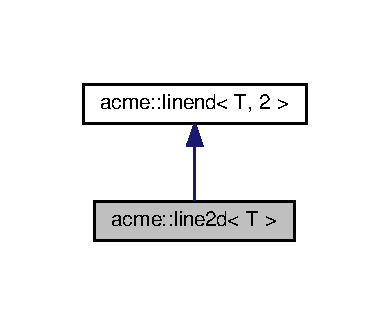
\includegraphics[width=187pt]{d0/d5c/classacme_1_1line2d__inherit__graph}
\end{center}
\end{figure}


Collaboration diagram for acme\+:\+:line2d$<$ T $>$\+:
\nopagebreak
\begin{figure}[H]
\begin{center}
\leavevmode
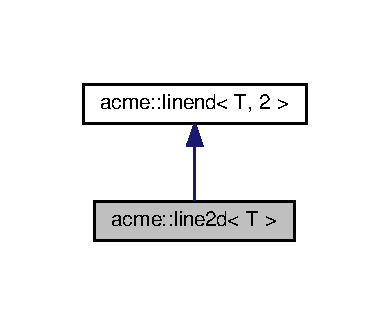
\includegraphics[width=187pt]{d0/d89/classacme_1_1line2d__coll__graph}
\end{center}
\end{figure}
\subsection*{Public Member Functions}
\begin{DoxyCompactItemize}
\item 
\mbox{\Hypertarget{classacme_1_1linend_a65c3e459b2a2b4768edfd4e550efce70}\label{classacme_1_1linend_a65c3e459b2a2b4768edfd4e550efce70}} 
\hyperlink{classacme_1_1pointnd}{pointnd}$<$ T, D $>$ \& {\bfseries operator\mbox{[}$\,$\mbox{]}} (const std\+::size\+\_\+t \&index)
\item 
\mbox{\Hypertarget{classacme_1_1linend_ac261d508a5222ae25402cab99e7befc5}\label{classacme_1_1linend_ac261d508a5222ae25402cab99e7befc5}} 
const \hyperlink{classacme_1_1pointnd}{pointnd}$<$ T, D $>$ \& {\bfseries operator\mbox{[}$\,$\mbox{]}} (const std\+::size\+\_\+t \&index) const
\item 
\mbox{\Hypertarget{classacme_1_1linend_ae00237c0a82ba7022922ca99c386df60}\label{classacme_1_1linend_ae00237c0a82ba7022922ca99c386df60}} 
std\+::size\+\_\+t {\bfseries size} ()
\end{DoxyCompactItemize}


The documentation for this class was generated from the following file\+:\begin{DoxyCompactItemize}
\item 
src/acme\+\_\+line.\+hh\end{DoxyCompactItemize}

\hypertarget{classacme_1_1line3d}{}\section{acme\+:\+:line3d$<$ T $>$ Class Template Reference}
\label{classacme_1_1line3d}\index{acme\+::line3d$<$ T $>$@{acme\+::line3d$<$ T $>$}}


Inheritance diagram for acme\+:\+:line3d$<$ T $>$\+:
\nopagebreak
\begin{figure}[H]
\begin{center}
\leavevmode
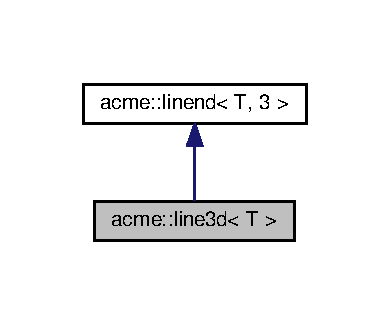
\includegraphics[width=187pt]{dd/d13/classacme_1_1line3d__inherit__graph}
\end{center}
\end{figure}


Collaboration diagram for acme\+:\+:line3d$<$ T $>$\+:
\nopagebreak
\begin{figure}[H]
\begin{center}
\leavevmode
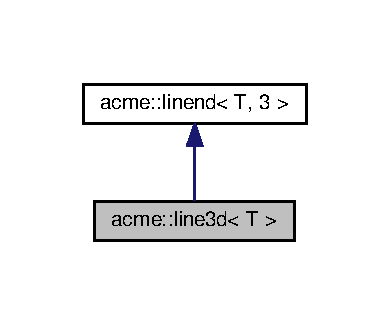
\includegraphics[width=187pt]{d9/d0d/classacme_1_1line3d__coll__graph}
\end{center}
\end{figure}
\subsection*{Public Member Functions}
\begin{DoxyCompactItemize}
\item 
\mbox{\Hypertarget{classacme_1_1linend_a65c3e459b2a2b4768edfd4e550efce70}\label{classacme_1_1linend_a65c3e459b2a2b4768edfd4e550efce70}} 
\hyperlink{classacme_1_1pointnd}{pointnd}$<$ T, D $>$ \& {\bfseries operator\mbox{[}$\,$\mbox{]}} (const std\+::size\+\_\+t \&index)
\item 
\mbox{\Hypertarget{classacme_1_1linend_ac261d508a5222ae25402cab99e7befc5}\label{classacme_1_1linend_ac261d508a5222ae25402cab99e7befc5}} 
const \hyperlink{classacme_1_1pointnd}{pointnd}$<$ T, D $>$ \& {\bfseries operator\mbox{[}$\,$\mbox{]}} (const std\+::size\+\_\+t \&index) const
\item 
\mbox{\Hypertarget{classacme_1_1linend_ae00237c0a82ba7022922ca99c386df60}\label{classacme_1_1linend_ae00237c0a82ba7022922ca99c386df60}} 
std\+::size\+\_\+t {\bfseries size} ()
\end{DoxyCompactItemize}


The documentation for this class was generated from the following file\+:\begin{DoxyCompactItemize}
\item 
src/acme\+\_\+line.\+hh\end{DoxyCompactItemize}

\hypertarget{classacme_1_1linend}{}\section{acme\+:\+:linend$<$ T, D $>$ Class Template Reference}
\label{classacme_1_1linend}\index{acme\+::linend$<$ T, D $>$@{acme\+::linend$<$ T, D $>$}}
\subsection*{Public Member Functions}
\begin{DoxyCompactItemize}
\item 
\mbox{\Hypertarget{classacme_1_1linend_a65c3e459b2a2b4768edfd4e550efce70}\label{classacme_1_1linend_a65c3e459b2a2b4768edfd4e550efce70}} 
\hyperlink{classacme_1_1pointnd}{pointnd}$<$ T, D $>$ \& {\bfseries operator\mbox{[}$\,$\mbox{]}} (const std\+::size\+\_\+t \&index)
\item 
\mbox{\Hypertarget{classacme_1_1linend_ac261d508a5222ae25402cab99e7befc5}\label{classacme_1_1linend_ac261d508a5222ae25402cab99e7befc5}} 
const \hyperlink{classacme_1_1pointnd}{pointnd}$<$ T, D $>$ \& {\bfseries operator\mbox{[}$\,$\mbox{]}} (const std\+::size\+\_\+t \&index) const
\item 
\mbox{\Hypertarget{classacme_1_1linend_ae00237c0a82ba7022922ca99c386df60}\label{classacme_1_1linend_ae00237c0a82ba7022922ca99c386df60}} 
std\+::size\+\_\+t {\bfseries size} ()
\end{DoxyCompactItemize}


The documentation for this class was generated from the following file\+:\begin{DoxyCompactItemize}
\item 
src/acme\+\_\+line.\+hh\end{DoxyCompactItemize}

\hypertarget{classacme_1_1point}{}\section{acme\+:\+:point$<$ T, D $>$ Class Template Reference}
\label{classacme_1_1point}\index{acme\+::point$<$ T, D $>$@{acme\+::point$<$ T, D $>$}}


The documentation for this class was generated from the following file\+:\begin{DoxyCompactItemize}
\item 
src/acme.\+hh\end{DoxyCompactItemize}

\hypertarget{classacme_1_1point2d}{}\section{acme\+:\+:point2d$<$ T $>$ Class Template Reference}
\label{classacme_1_1point2d}\index{acme\+::point2d$<$ T $>$@{acme\+::point2d$<$ T $>$}}


2-\/dimensional point class container  




{\ttfamily \#include $<$acme\+\_\+point.\+hh$>$}



Inheritance diagram for acme\+:\+:point2d$<$ T $>$\+:
\nopagebreak
\begin{figure}[H]
\begin{center}
\leavevmode
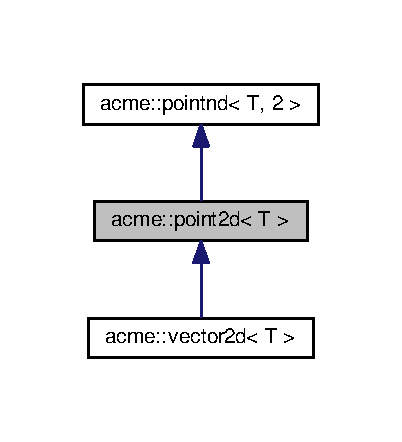
\includegraphics[width=193pt]{d9/d99/classacme_1_1point2d__inherit__graph}
\end{center}
\end{figure}


Collaboration diagram for acme\+:\+:point2d$<$ T $>$\+:
\nopagebreak
\begin{figure}[H]
\begin{center}
\leavevmode
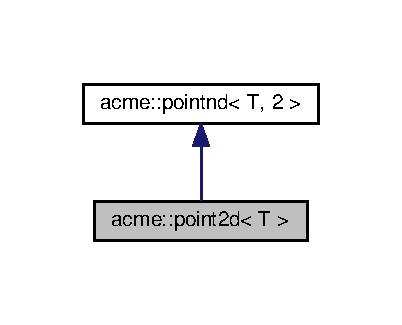
\includegraphics[width=193pt]{d9/da9/classacme_1_1point2d__coll__graph}
\end{center}
\end{figure}
\subsection*{Public Member Functions}
\begin{DoxyCompactItemize}
\item 
\mbox{\Hypertarget{classacme_1_1point2d_a1ebb66adbd7754b28e42a7049f09f12a}\label{classacme_1_1point2d_a1ebb66adbd7754b28e42a7049f09f12a}} 
\hyperlink{classacme_1_1point2d_a1ebb66adbd7754b28e42a7049f09f12a}{point2d} ()
\begin{DoxyCompactList}\small\item\em Class constructor. \end{DoxyCompactList}\item 
\hyperlink{classacme_1_1point2d_a850b6a667ca69c35114ac1ec83a68f2d}{point2d} (const T \&value0, const T \&value1)
\begin{DoxyCompactList}\small\item\em Class constructor. \end{DoxyCompactList}\item 
\hyperlink{classacme_1_1point2d_a01471e5d6f2b7e1851499a9d16187ea5}{point2d} (const \hyperlink{classacme_1_1pointnd}{pointnd}$<$ T, 2 $>$ \&\hyperlink{classacme_1_1point}{point})
\begin{DoxyCompactList}\small\item\em Class constructor. \end{DoxyCompactList}\item 
\hyperlink{classacme_1_1point2d_aa13d8e0048a9936b017fe8e0f4f5cdf4}{point2d} (const \hyperlink{classacme_1_1point2d}{point2d}$<$ T $>$ \&\hyperlink{classacme_1_1point}{point})
\begin{DoxyCompactList}\small\item\em Class constructor. \end{DoxyCompactList}\item 
\mbox{\Hypertarget{classacme_1_1point2d_ae1e790b48d7cb9b6f8e29142c4b3d51f}\label{classacme_1_1point2d_ae1e790b48d7cb9b6f8e29142c4b3d51f}} 
\hyperlink{classacme_1_1point2d_ae1e790b48d7cb9b6f8e29142c4b3d51f}{$\sim$point2d} ()
\begin{DoxyCompactList}\small\item\em Class destructor. \end{DoxyCompactList}\item 
\hyperlink{classacme_1_1point2d}{point2d}$<$ T $>$ \& \hyperlink{classacme_1_1point2d_a1032b0e98d229f2d6d59aba5514b3c2f}{operator=} (const \hyperlink{classacme_1_1pointnd}{pointnd}$<$ T, 2 $>$ \&\hyperlink{classacme_1_1point}{point})
\begin{DoxyCompactList}\small\item\em Equality operator. \end{DoxyCompactList}\item 
\mbox{\Hypertarget{classacme_1_1point2d_aa62c36149dc319bcd38b351be5230f04}\label{classacme_1_1point2d_aa62c36149dc319bcd38b351be5230f04}} 
const T \& \hyperlink{classacme_1_1point2d_aa62c36149dc319bcd38b351be5230f04}{x} () const
\begin{DoxyCompactList}\small\item\em Getter for point x value. \end{DoxyCompactList}\item 
\mbox{\Hypertarget{classacme_1_1point2d_adf79b9f2fbcac2c5f1bea2bece0e9b27}\label{classacme_1_1point2d_adf79b9f2fbcac2c5f1bea2bece0e9b27}} 
const T \& \hyperlink{classacme_1_1point2d_adf79b9f2fbcac2c5f1bea2bece0e9b27}{y} () const
\begin{DoxyCompactList}\small\item\em Getter for point y value. \end{DoxyCompactList}\item 
void \hyperlink{classacme_1_1point2d_a158797a6603451c35bd0e2be3be3b2c8}{x} (const T \&x)
\begin{DoxyCompactList}\small\item\em Setter for point x value. \end{DoxyCompactList}\item 
void \hyperlink{classacme_1_1point2d_ab1baab0e82e178f1e828a25fa8dbb1c8}{y} (const T \&y)
\begin{DoxyCompactList}\small\item\em Setter for point y value. \end{DoxyCompactList}\item 
\hyperlink{classacme_1_1point2d}{point2d}$<$ T $>$ \& \hyperlink{classacme_1_1point2d_a23948fcd0635557e8eeb0c298bb96f68}{make3dX} (const T \&\hyperlink{classacme_1_1point2d_aa62c36149dc319bcd38b351be5230f04}{x})
\begin{DoxyCompactList}\small\item\em Create a 3-\/dimensional point by addind x value. \end{DoxyCompactList}\item 
\hyperlink{classacme_1_1point2d}{point2d}$<$ T $>$ \& \hyperlink{classacme_1_1point2d_ac6bdbcec56da64ea0265691f3e734625}{make3dY} (const T \&\hyperlink{classacme_1_1point2d_adf79b9f2fbcac2c5f1bea2bece0e9b27}{y})
\begin{DoxyCompactList}\small\item\em Create a 3-\/dimensional point by addind y value. \end{DoxyCompactList}\item 
\hyperlink{classacme_1_1point2d}{point2d}$<$ T $>$ \& \hyperlink{classacme_1_1point2d_a605f4d335747c08026316ec4982b7eb5}{make3dZ} (const T \&z)
\begin{DoxyCompactList}\small\item\em Create a 3-\/dimensional point by addind z value. \end{DoxyCompactList}\item 
\mbox{\Hypertarget{classacme_1_1pointnd_a2d0b84e609dc1ad5cbbe631c5bb5791f}\label{classacme_1_1pointnd_a2d0b84e609dc1ad5cbbe631c5bb5791f}} 
void \hyperlink{classacme_1_1pointnd_a2d0b84e609dc1ad5cbbe631c5bb5791f}{clear} ()
\begin{DoxyCompactList}\small\item\em Clear vector data. \end{DoxyCompactList}\item 
T \& \hyperlink{classacme_1_1pointnd_a35b0691673728d98d455c007612d6b91}{operator\mbox{[}$\,$\mbox{]}} (const std\+::size\+\_\+t \&index)
\begin{DoxyCompactList}\small\item\em Indexing operator. \end{DoxyCompactList}\item 
const T \& \hyperlink{classacme_1_1pointnd_a565e9ed195c8f8dadc570a029a3deb94}{operator\mbox{[}$\,$\mbox{]}} (const std\+::size\+\_\+t \&index) const
\begin{DoxyCompactList}\small\item\em Indexing operator. \end{DoxyCompactList}\end{DoxyCompactItemize}
\subsection*{Protected Attributes}
\begin{DoxyCompactItemize}
\item 
\mbox{\Hypertarget{classacme_1_1pointnd_a13b19080ed617e2a9c5d6058f07d4f4b}\label{classacme_1_1pointnd_a13b19080ed617e2a9c5d6058f07d4f4b}} 
Eigen\+::\+Matrix$<$ T, D, 1 $>$ {\bfseries data}
\end{DoxyCompactItemize}


\subsection{Detailed Description}
\subsubsection*{template$<$typename T = Float$>$\newline
class acme\+::point2d$<$ T $>$}

2-\/dimensional point class container 

\subsection{Constructor \& Destructor Documentation}
\mbox{\Hypertarget{classacme_1_1point2d_a850b6a667ca69c35114ac1ec83a68f2d}\label{classacme_1_1point2d_a850b6a667ca69c35114ac1ec83a68f2d}} 
\index{acme\+::point2d@{acme\+::point2d}!point2d@{point2d}}
\index{point2d@{point2d}!acme\+::point2d@{acme\+::point2d}}
\subsubsection{\texorpdfstring{point2d()}{point2d()}\hspace{0.1cm}{\footnotesize\ttfamily [1/3]}}
{\footnotesize\ttfamily template$<$typename T = Float$>$ \\
\hyperlink{classacme_1_1point2d}{acme\+::point2d}$<$ T $>$\+::\hyperlink{classacme_1_1point2d}{point2d} (\begin{DoxyParamCaption}\item[{const T \&}]{value0,  }\item[{const T \&}]{value1 }\end{DoxyParamCaption})\hspace{0.3cm}{\ttfamily [inline]}}



Class constructor. 


\begin{DoxyParams}{Parameters}
{\em value0} & Input value 0 \\
\hline
{\em value1} & Input value 1 \\
\hline
\end{DoxyParams}
\mbox{\Hypertarget{classacme_1_1point2d_a01471e5d6f2b7e1851499a9d16187ea5}\label{classacme_1_1point2d_a01471e5d6f2b7e1851499a9d16187ea5}} 
\index{acme\+::point2d@{acme\+::point2d}!point2d@{point2d}}
\index{point2d@{point2d}!acme\+::point2d@{acme\+::point2d}}
\subsubsection{\texorpdfstring{point2d()}{point2d()}\hspace{0.1cm}{\footnotesize\ttfamily [2/3]}}
{\footnotesize\ttfamily template$<$typename T = Float$>$ \\
\hyperlink{classacme_1_1point2d}{acme\+::point2d}$<$ T $>$\+::\hyperlink{classacme_1_1point2d}{point2d} (\begin{DoxyParamCaption}\item[{const \hyperlink{classacme_1_1pointnd}{pointnd}$<$ T, 2 $>$ \&}]{point }\end{DoxyParamCaption})\hspace{0.3cm}{\ttfamily [inline]}}



Class constructor. 


\begin{DoxyParams}{Parameters}
{\em point} & Input 2-\/dimensional point \\
\hline
\end{DoxyParams}
\mbox{\Hypertarget{classacme_1_1point2d_aa13d8e0048a9936b017fe8e0f4f5cdf4}\label{classacme_1_1point2d_aa13d8e0048a9936b017fe8e0f4f5cdf4}} 
\index{acme\+::point2d@{acme\+::point2d}!point2d@{point2d}}
\index{point2d@{point2d}!acme\+::point2d@{acme\+::point2d}}
\subsubsection{\texorpdfstring{point2d()}{point2d()}\hspace{0.1cm}{\footnotesize\ttfamily [3/3]}}
{\footnotesize\ttfamily template$<$typename T = Float$>$ \\
\hyperlink{classacme_1_1point2d}{acme\+::point2d}$<$ T $>$\+::\hyperlink{classacme_1_1point2d}{point2d} (\begin{DoxyParamCaption}\item[{const \hyperlink{classacme_1_1point2d}{point2d}$<$ T $>$ \&}]{point }\end{DoxyParamCaption})\hspace{0.3cm}{\ttfamily [inline]}}



Class constructor. 


\begin{DoxyParams}{Parameters}
{\em point} & Input 2-\/dimensional point \\
\hline
\end{DoxyParams}


\subsection{Member Function Documentation}
\mbox{\Hypertarget{classacme_1_1point2d_a23948fcd0635557e8eeb0c298bb96f68}\label{classacme_1_1point2d_a23948fcd0635557e8eeb0c298bb96f68}} 
\index{acme\+::point2d@{acme\+::point2d}!make3dX@{make3dX}}
\index{make3dX@{make3dX}!acme\+::point2d@{acme\+::point2d}}
\subsubsection{\texorpdfstring{make3d\+X()}{make3dX()}}
{\footnotesize\ttfamily template$<$typename T = Float$>$ \\
\hyperlink{classacme_1_1point2d}{point2d}$<$T$>$\& \hyperlink{classacme_1_1point2d}{acme\+::point2d}$<$ T $>$\+::make3dX (\begin{DoxyParamCaption}\item[{const T \&}]{x }\end{DoxyParamCaption})\hspace{0.3cm}{\ttfamily [inline]}}



Create a 3-\/dimensional point by addind x value. 


\begin{DoxyParams}{Parameters}
{\em x} & Input x value \\
\hline
\end{DoxyParams}
\mbox{\Hypertarget{classacme_1_1point2d_ac6bdbcec56da64ea0265691f3e734625}\label{classacme_1_1point2d_ac6bdbcec56da64ea0265691f3e734625}} 
\index{acme\+::point2d@{acme\+::point2d}!make3dY@{make3dY}}
\index{make3dY@{make3dY}!acme\+::point2d@{acme\+::point2d}}
\subsubsection{\texorpdfstring{make3d\+Y()}{make3dY()}}
{\footnotesize\ttfamily template$<$typename T = Float$>$ \\
\hyperlink{classacme_1_1point2d}{point2d}$<$T$>$\& \hyperlink{classacme_1_1point2d}{acme\+::point2d}$<$ T $>$\+::make3dY (\begin{DoxyParamCaption}\item[{const T \&}]{y }\end{DoxyParamCaption})\hspace{0.3cm}{\ttfamily [inline]}}



Create a 3-\/dimensional point by addind y value. 


\begin{DoxyParams}{Parameters}
{\em y} & Input y value \\
\hline
\end{DoxyParams}
\mbox{\Hypertarget{classacme_1_1point2d_a605f4d335747c08026316ec4982b7eb5}\label{classacme_1_1point2d_a605f4d335747c08026316ec4982b7eb5}} 
\index{acme\+::point2d@{acme\+::point2d}!make3dZ@{make3dZ}}
\index{make3dZ@{make3dZ}!acme\+::point2d@{acme\+::point2d}}
\subsubsection{\texorpdfstring{make3d\+Z()}{make3dZ()}}
{\footnotesize\ttfamily template$<$typename T = Float$>$ \\
\hyperlink{classacme_1_1point2d}{point2d}$<$T$>$\& \hyperlink{classacme_1_1point2d}{acme\+::point2d}$<$ T $>$\+::make3dZ (\begin{DoxyParamCaption}\item[{const T \&}]{z }\end{DoxyParamCaption})\hspace{0.3cm}{\ttfamily [inline]}}



Create a 3-\/dimensional point by addind z value. 


\begin{DoxyParams}{Parameters}
{\em z} & Input z value \\
\hline
\end{DoxyParams}
\mbox{\Hypertarget{classacme_1_1point2d_a1032b0e98d229f2d6d59aba5514b3c2f}\label{classacme_1_1point2d_a1032b0e98d229f2d6d59aba5514b3c2f}} 
\index{acme\+::point2d@{acme\+::point2d}!operator=@{operator=}}
\index{operator=@{operator=}!acme\+::point2d@{acme\+::point2d}}
\subsubsection{\texorpdfstring{operator=()}{operator=()}}
{\footnotesize\ttfamily template$<$typename T = Float$>$ \\
\hyperlink{classacme_1_1point2d}{point2d}$<$T$>$\& \hyperlink{classacme_1_1point2d}{acme\+::point2d}$<$ T $>$\+::operator= (\begin{DoxyParamCaption}\item[{const \hyperlink{classacme_1_1pointnd}{pointnd}$<$ T, 2 $>$ \&}]{point }\end{DoxyParamCaption})\hspace{0.3cm}{\ttfamily [inline]}}



Equality operator. 


\begin{DoxyParams}{Parameters}
{\em point} & Input 2-\/dimensional point \\
\hline
\end{DoxyParams}
\mbox{\Hypertarget{classacme_1_1pointnd_a35b0691673728d98d455c007612d6b91}\label{classacme_1_1pointnd_a35b0691673728d98d455c007612d6b91}} 
\index{acme\+::point2d@{acme\+::point2d}!operator\mbox{[}\mbox{]}@{operator[]}}
\index{operator\mbox{[}\mbox{]}@{operator[]}!acme\+::point2d@{acme\+::point2d}}
\subsubsection{\texorpdfstring{operator[]()}{operator[]()}\hspace{0.1cm}{\footnotesize\ttfamily [1/2]}}
{\footnotesize\ttfamily T\& \hyperlink{classacme_1_1pointnd}{acme\+::pointnd}$<$ T, D $>$\+::operator\mbox{[}$\,$\mbox{]} (\begin{DoxyParamCaption}\item[{const std\+::size\+\_\+t \&}]{index }\end{DoxyParamCaption})\hspace{0.3cm}{\ttfamily [inline]}, {\ttfamily [inherited]}}



Indexing operator. 


\begin{DoxyParams}{Parameters}
{\em index} & Input index \\
\hline
\end{DoxyParams}
\mbox{\Hypertarget{classacme_1_1pointnd_a565e9ed195c8f8dadc570a029a3deb94}\label{classacme_1_1pointnd_a565e9ed195c8f8dadc570a029a3deb94}} 
\index{acme\+::point2d@{acme\+::point2d}!operator\mbox{[}\mbox{]}@{operator[]}}
\index{operator\mbox{[}\mbox{]}@{operator[]}!acme\+::point2d@{acme\+::point2d}}
\subsubsection{\texorpdfstring{operator[]()}{operator[]()}\hspace{0.1cm}{\footnotesize\ttfamily [2/2]}}
{\footnotesize\ttfamily const T\& \hyperlink{classacme_1_1pointnd}{acme\+::pointnd}$<$ T, D $>$\+::operator\mbox{[}$\,$\mbox{]} (\begin{DoxyParamCaption}\item[{const std\+::size\+\_\+t \&}]{index }\end{DoxyParamCaption}) const\hspace{0.3cm}{\ttfamily [inline]}, {\ttfamily [inherited]}}



Indexing operator. 


\begin{DoxyParams}{Parameters}
{\em index} & Input index \\
\hline
\end{DoxyParams}
\mbox{\Hypertarget{classacme_1_1point2d_a158797a6603451c35bd0e2be3be3b2c8}\label{classacme_1_1point2d_a158797a6603451c35bd0e2be3be3b2c8}} 
\index{acme\+::point2d@{acme\+::point2d}!x@{x}}
\index{x@{x}!acme\+::point2d@{acme\+::point2d}}
\subsubsection{\texorpdfstring{x()}{x()}}
{\footnotesize\ttfamily template$<$typename T = Float$>$ \\
void \hyperlink{classacme_1_1point2d}{acme\+::point2d}$<$ T $>$\+::x (\begin{DoxyParamCaption}\item[{const T \&}]{x }\end{DoxyParamCaption})\hspace{0.3cm}{\ttfamily [inline]}}



Setter for point x value. 


\begin{DoxyParams}{Parameters}
{\em x} & Input x value \\
\hline
\end{DoxyParams}
\mbox{\Hypertarget{classacme_1_1point2d_ab1baab0e82e178f1e828a25fa8dbb1c8}\label{classacme_1_1point2d_ab1baab0e82e178f1e828a25fa8dbb1c8}} 
\index{acme\+::point2d@{acme\+::point2d}!y@{y}}
\index{y@{y}!acme\+::point2d@{acme\+::point2d}}
\subsubsection{\texorpdfstring{y()}{y()}}
{\footnotesize\ttfamily template$<$typename T = Float$>$ \\
void \hyperlink{classacme_1_1point2d}{acme\+::point2d}$<$ T $>$\+::y (\begin{DoxyParamCaption}\item[{const T \&}]{y }\end{DoxyParamCaption})\hspace{0.3cm}{\ttfamily [inline]}}



Setter for point y value. 


\begin{DoxyParams}{Parameters}
{\em y} & Input y value \\
\hline
\end{DoxyParams}


The documentation for this class was generated from the following file\+:\begin{DoxyCompactItemize}
\item 
src/acme\+\_\+point.\+hh\end{DoxyCompactItemize}

\hypertarget{classacme_1_1point3d}{}\section{acme\+:\+:point3d$<$ T $>$ Class Template Reference}
\label{classacme_1_1point3d}\index{acme\+::point3d$<$ T $>$@{acme\+::point3d$<$ T $>$}}


3-\/dimensional point class container  




{\ttfamily \#include $<$acme\+\_\+point.\+hh$>$}



Inheritance diagram for acme\+:\+:point3d$<$ T $>$\+:
\nopagebreak
\begin{figure}[H]
\begin{center}
\leavevmode
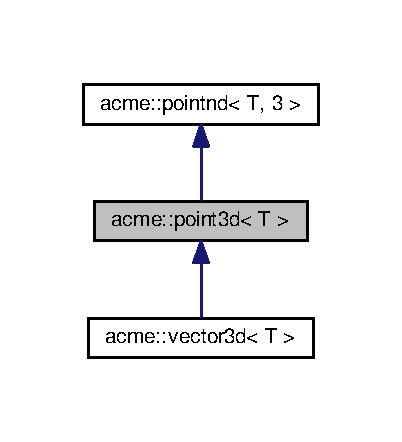
\includegraphics[width=193pt]{dc/d40/classacme_1_1point3d__inherit__graph}
\end{center}
\end{figure}


Collaboration diagram for acme\+:\+:point3d$<$ T $>$\+:
\nopagebreak
\begin{figure}[H]
\begin{center}
\leavevmode
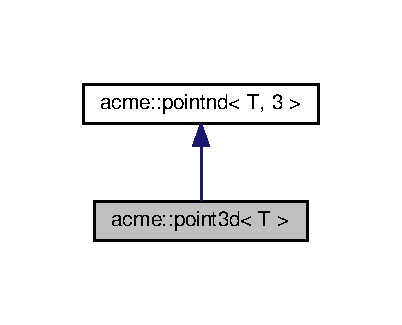
\includegraphics[width=193pt]{d9/d61/classacme_1_1point3d__coll__graph}
\end{center}
\end{figure}
\subsection*{Public Member Functions}
\begin{DoxyCompactItemize}
\item 
\mbox{\Hypertarget{classacme_1_1point3d_a6c02c53c7b8bd7d182e4a30e33bb3651}\label{classacme_1_1point3d_a6c02c53c7b8bd7d182e4a30e33bb3651}} 
\hyperlink{classacme_1_1point3d_a6c02c53c7b8bd7d182e4a30e33bb3651}{point3d} ()
\begin{DoxyCompactList}\small\item\em Class constructor. \end{DoxyCompactList}\item 
\hyperlink{classacme_1_1point3d_a11ad282f54092ff2b4cd440722268c07}{point3d} (const T \&value0, const T \&value1, const T \&value2)
\begin{DoxyCompactList}\small\item\em Class constructor. \end{DoxyCompactList}\item 
\hyperlink{classacme_1_1point3d_ad8106a84822af4431c6b899656e3af06}{point3d} (const \hyperlink{classacme_1_1pointnd}{pointnd}$<$ T, 3 $>$ \&\hyperlink{classacme_1_1point}{point})
\begin{DoxyCompactList}\small\item\em Class constructor. \end{DoxyCompactList}\item 
\hyperlink{classacme_1_1point3d_abd49fc12054b5a19c13973f9d0abcf3d}{point3d} (const \hyperlink{classacme_1_1point3d}{point3d}$<$ T $>$ \&\hyperlink{classacme_1_1point}{point})
\begin{DoxyCompactList}\small\item\em Class constructor. \end{DoxyCompactList}\item 
\mbox{\Hypertarget{classacme_1_1point3d_a2f2bb6249494c61c600aaa37f674d864}\label{classacme_1_1point3d_a2f2bb6249494c61c600aaa37f674d864}} 
\hyperlink{classacme_1_1point3d_a2f2bb6249494c61c600aaa37f674d864}{$\sim$point3d} ()
\begin{DoxyCompactList}\small\item\em Class destructor. \end{DoxyCompactList}\item 
\hyperlink{classacme_1_1point3d}{point3d}$<$ T $>$ \& \hyperlink{classacme_1_1point3d_ae4d80a128a282ef6b98560c5932abe13}{operator=} (const \hyperlink{classacme_1_1pointnd}{pointnd}$<$ T, 3 $>$ \&\hyperlink{classacme_1_1point}{point})
\begin{DoxyCompactList}\small\item\em Equality operator. \end{DoxyCompactList}\item 
\mbox{\Hypertarget{classacme_1_1point3d_a7ace84b8e85e0762e8c900ef7dfabf61}\label{classacme_1_1point3d_a7ace84b8e85e0762e8c900ef7dfabf61}} 
const T \& \hyperlink{classacme_1_1point3d_a7ace84b8e85e0762e8c900ef7dfabf61}{x} () const
\begin{DoxyCompactList}\small\item\em Getter for point x value. \end{DoxyCompactList}\item 
\mbox{\Hypertarget{classacme_1_1point3d_a1a13aea2bb5e756c74ca6187e4b927d2}\label{classacme_1_1point3d_a1a13aea2bb5e756c74ca6187e4b927d2}} 
const T \& \hyperlink{classacme_1_1point3d_a1a13aea2bb5e756c74ca6187e4b927d2}{y} () const
\begin{DoxyCompactList}\small\item\em Getter for point y value. \end{DoxyCompactList}\item 
\mbox{\Hypertarget{classacme_1_1point3d_acbea0b411604f8da4f690e09e2401743}\label{classacme_1_1point3d_acbea0b411604f8da4f690e09e2401743}} 
const T \& \hyperlink{classacme_1_1point3d_acbea0b411604f8da4f690e09e2401743}{z} () const
\begin{DoxyCompactList}\small\item\em Getter for point z value. \end{DoxyCompactList}\item 
void \hyperlink{classacme_1_1point3d_acccc28f082747904be0f39bd5972a40e}{x} (const T \&x)
\begin{DoxyCompactList}\small\item\em Setter for point x value. \end{DoxyCompactList}\item 
void \hyperlink{classacme_1_1point3d_ad9b058b4ba5ca4172a8c4ded27c89825}{y} (const T \&y)
\begin{DoxyCompactList}\small\item\em Setter for point y value. \end{DoxyCompactList}\item 
void \hyperlink{classacme_1_1point3d_aad69f4d32ffafffd008214c361fa843f}{z} (const T \&z)
\begin{DoxyCompactList}\small\item\em Setter for point z value. \end{DoxyCompactList}\item 
\hyperlink{classacme_1_1point2d}{point2d}$<$ T $>$ \& \hyperlink{classacme_1_1point3d_a724a96c6ad4aa84b0236a8113d99d4a4}{make2d} (const std\+::size\+\_\+t \&index1, const std\+::size\+\_\+t \&index2)
\begin{DoxyCompactList}\small\item\em Create a 3-\/dimensional point by addind value on selected index value. \end{DoxyCompactList}\item 
\mbox{\Hypertarget{classacme_1_1pointnd_a2d0b84e609dc1ad5cbbe631c5bb5791f}\label{classacme_1_1pointnd_a2d0b84e609dc1ad5cbbe631c5bb5791f}} 
void \hyperlink{classacme_1_1pointnd_a2d0b84e609dc1ad5cbbe631c5bb5791f}{clear} ()
\begin{DoxyCompactList}\small\item\em Clear vector data. \end{DoxyCompactList}\item 
T \& \hyperlink{classacme_1_1pointnd_a35b0691673728d98d455c007612d6b91}{operator\mbox{[}$\,$\mbox{]}} (const std\+::size\+\_\+t \&index)
\begin{DoxyCompactList}\small\item\em Indexing operator. \end{DoxyCompactList}\item 
const T \& \hyperlink{classacme_1_1pointnd_a565e9ed195c8f8dadc570a029a3deb94}{operator\mbox{[}$\,$\mbox{]}} (const std\+::size\+\_\+t \&index) const
\begin{DoxyCompactList}\small\item\em Indexing operator. \end{DoxyCompactList}\end{DoxyCompactItemize}
\subsection*{Protected Attributes}
\begin{DoxyCompactItemize}
\item 
\mbox{\Hypertarget{classacme_1_1pointnd_a13b19080ed617e2a9c5d6058f07d4f4b}\label{classacme_1_1pointnd_a13b19080ed617e2a9c5d6058f07d4f4b}} 
Eigen\+::\+Matrix$<$ T, D, 1 $>$ {\bfseries data}
\end{DoxyCompactItemize}


\subsection{Detailed Description}
\subsubsection*{template$<$typename T = Float$>$\newline
class acme\+::point3d$<$ T $>$}

3-\/dimensional point class container 

\subsection{Constructor \& Destructor Documentation}
\mbox{\Hypertarget{classacme_1_1point3d_a11ad282f54092ff2b4cd440722268c07}\label{classacme_1_1point3d_a11ad282f54092ff2b4cd440722268c07}} 
\index{acme\+::point3d@{acme\+::point3d}!point3d@{point3d}}
\index{point3d@{point3d}!acme\+::point3d@{acme\+::point3d}}
\subsubsection{\texorpdfstring{point3d()}{point3d()}\hspace{0.1cm}{\footnotesize\ttfamily [1/3]}}
{\footnotesize\ttfamily template$<$typename T = Float$>$ \\
\hyperlink{classacme_1_1point3d}{acme\+::point3d}$<$ T $>$\+::\hyperlink{classacme_1_1point3d}{point3d} (\begin{DoxyParamCaption}\item[{const T \&}]{value0,  }\item[{const T \&}]{value1,  }\item[{const T \&}]{value2 }\end{DoxyParamCaption})\hspace{0.3cm}{\ttfamily [inline]}}



Class constructor. 


\begin{DoxyParams}{Parameters}
{\em value0} & Input value 0 \\
\hline
{\em value1} & Input value 1 \\
\hline
{\em value2} & Input value 2 \\
\hline
\end{DoxyParams}
\mbox{\Hypertarget{classacme_1_1point3d_ad8106a84822af4431c6b899656e3af06}\label{classacme_1_1point3d_ad8106a84822af4431c6b899656e3af06}} 
\index{acme\+::point3d@{acme\+::point3d}!point3d@{point3d}}
\index{point3d@{point3d}!acme\+::point3d@{acme\+::point3d}}
\subsubsection{\texorpdfstring{point3d()}{point3d()}\hspace{0.1cm}{\footnotesize\ttfamily [2/3]}}
{\footnotesize\ttfamily template$<$typename T = Float$>$ \\
\hyperlink{classacme_1_1point3d}{acme\+::point3d}$<$ T $>$\+::\hyperlink{classacme_1_1point3d}{point3d} (\begin{DoxyParamCaption}\item[{const \hyperlink{classacme_1_1pointnd}{pointnd}$<$ T, 3 $>$ \&}]{point }\end{DoxyParamCaption})\hspace{0.3cm}{\ttfamily [inline]}}



Class constructor. 


\begin{DoxyParams}{Parameters}
{\em point} & Input 3-\/dimensional point \\
\hline
\end{DoxyParams}
\mbox{\Hypertarget{classacme_1_1point3d_abd49fc12054b5a19c13973f9d0abcf3d}\label{classacme_1_1point3d_abd49fc12054b5a19c13973f9d0abcf3d}} 
\index{acme\+::point3d@{acme\+::point3d}!point3d@{point3d}}
\index{point3d@{point3d}!acme\+::point3d@{acme\+::point3d}}
\subsubsection{\texorpdfstring{point3d()}{point3d()}\hspace{0.1cm}{\footnotesize\ttfamily [3/3]}}
{\footnotesize\ttfamily template$<$typename T = Float$>$ \\
\hyperlink{classacme_1_1point3d}{acme\+::point3d}$<$ T $>$\+::\hyperlink{classacme_1_1point3d}{point3d} (\begin{DoxyParamCaption}\item[{const \hyperlink{classacme_1_1point3d}{point3d}$<$ T $>$ \&}]{point }\end{DoxyParamCaption})\hspace{0.3cm}{\ttfamily [inline]}}



Class constructor. 


\begin{DoxyParams}{Parameters}
{\em point} & Input 3-\/dimensional point \\
\hline
\end{DoxyParams}


\subsection{Member Function Documentation}
\mbox{\Hypertarget{classacme_1_1point3d_a724a96c6ad4aa84b0236a8113d99d4a4}\label{classacme_1_1point3d_a724a96c6ad4aa84b0236a8113d99d4a4}} 
\index{acme\+::point3d@{acme\+::point3d}!make2d@{make2d}}
\index{make2d@{make2d}!acme\+::point3d@{acme\+::point3d}}
\subsubsection{\texorpdfstring{make2d()}{make2d()}}
{\footnotesize\ttfamily template$<$typename T = Float$>$ \\
\hyperlink{classacme_1_1point2d}{point2d}$<$T$>$\& \hyperlink{classacme_1_1point3d}{acme\+::point3d}$<$ T $>$\+::make2d (\begin{DoxyParamCaption}\item[{const std\+::size\+\_\+t \&}]{index1,  }\item[{const std\+::size\+\_\+t \&}]{index2 }\end{DoxyParamCaption})\hspace{0.3cm}{\ttfamily [inline]}}



Create a 3-\/dimensional point by addind value on selected index value. 


\begin{DoxyParams}{Parameters}
{\em index1} & Inuput index 1 \\
\hline
{\em index2} & Inuput index 2 \\
\hline
\end{DoxyParams}
\mbox{\Hypertarget{classacme_1_1point3d_ae4d80a128a282ef6b98560c5932abe13}\label{classacme_1_1point3d_ae4d80a128a282ef6b98560c5932abe13}} 
\index{acme\+::point3d@{acme\+::point3d}!operator=@{operator=}}
\index{operator=@{operator=}!acme\+::point3d@{acme\+::point3d}}
\subsubsection{\texorpdfstring{operator=()}{operator=()}}
{\footnotesize\ttfamily template$<$typename T = Float$>$ \\
\hyperlink{classacme_1_1point3d}{point3d}$<$T$>$\& \hyperlink{classacme_1_1point3d}{acme\+::point3d}$<$ T $>$\+::operator= (\begin{DoxyParamCaption}\item[{const \hyperlink{classacme_1_1pointnd}{pointnd}$<$ T, 3 $>$ \&}]{point }\end{DoxyParamCaption})\hspace{0.3cm}{\ttfamily [inline]}}



Equality operator. 


\begin{DoxyParams}{Parameters}
{\em point} & Input 3-\/dimensional point \\
\hline
\end{DoxyParams}
\mbox{\Hypertarget{classacme_1_1pointnd_a35b0691673728d98d455c007612d6b91}\label{classacme_1_1pointnd_a35b0691673728d98d455c007612d6b91}} 
\index{acme\+::point3d@{acme\+::point3d}!operator\mbox{[}\mbox{]}@{operator[]}}
\index{operator\mbox{[}\mbox{]}@{operator[]}!acme\+::point3d@{acme\+::point3d}}
\subsubsection{\texorpdfstring{operator[]()}{operator[]()}\hspace{0.1cm}{\footnotesize\ttfamily [1/2]}}
{\footnotesize\ttfamily T\& \hyperlink{classacme_1_1pointnd}{acme\+::pointnd}$<$ T, D $>$\+::operator\mbox{[}$\,$\mbox{]} (\begin{DoxyParamCaption}\item[{const std\+::size\+\_\+t \&}]{index }\end{DoxyParamCaption})\hspace{0.3cm}{\ttfamily [inline]}, {\ttfamily [inherited]}}



Indexing operator. 


\begin{DoxyParams}{Parameters}
{\em index} & Input index \\
\hline
\end{DoxyParams}
\mbox{\Hypertarget{classacme_1_1pointnd_a565e9ed195c8f8dadc570a029a3deb94}\label{classacme_1_1pointnd_a565e9ed195c8f8dadc570a029a3deb94}} 
\index{acme\+::point3d@{acme\+::point3d}!operator\mbox{[}\mbox{]}@{operator[]}}
\index{operator\mbox{[}\mbox{]}@{operator[]}!acme\+::point3d@{acme\+::point3d}}
\subsubsection{\texorpdfstring{operator[]()}{operator[]()}\hspace{0.1cm}{\footnotesize\ttfamily [2/2]}}
{\footnotesize\ttfamily const T\& \hyperlink{classacme_1_1pointnd}{acme\+::pointnd}$<$ T, D $>$\+::operator\mbox{[}$\,$\mbox{]} (\begin{DoxyParamCaption}\item[{const std\+::size\+\_\+t \&}]{index }\end{DoxyParamCaption}) const\hspace{0.3cm}{\ttfamily [inline]}, {\ttfamily [inherited]}}



Indexing operator. 


\begin{DoxyParams}{Parameters}
{\em index} & Input index \\
\hline
\end{DoxyParams}
\mbox{\Hypertarget{classacme_1_1point3d_acccc28f082747904be0f39bd5972a40e}\label{classacme_1_1point3d_acccc28f082747904be0f39bd5972a40e}} 
\index{acme\+::point3d@{acme\+::point3d}!x@{x}}
\index{x@{x}!acme\+::point3d@{acme\+::point3d}}
\subsubsection{\texorpdfstring{x()}{x()}}
{\footnotesize\ttfamily template$<$typename T = Float$>$ \\
void \hyperlink{classacme_1_1point3d}{acme\+::point3d}$<$ T $>$\+::x (\begin{DoxyParamCaption}\item[{const T \&}]{x }\end{DoxyParamCaption})\hspace{0.3cm}{\ttfamily [inline]}}



Setter for point x value. 


\begin{DoxyParams}{Parameters}
{\em x} & Input x value \\
\hline
\end{DoxyParams}
\mbox{\Hypertarget{classacme_1_1point3d_ad9b058b4ba5ca4172a8c4ded27c89825}\label{classacme_1_1point3d_ad9b058b4ba5ca4172a8c4ded27c89825}} 
\index{acme\+::point3d@{acme\+::point3d}!y@{y}}
\index{y@{y}!acme\+::point3d@{acme\+::point3d}}
\subsubsection{\texorpdfstring{y()}{y()}}
{\footnotesize\ttfamily template$<$typename T = Float$>$ \\
void \hyperlink{classacme_1_1point3d}{acme\+::point3d}$<$ T $>$\+::y (\begin{DoxyParamCaption}\item[{const T \&}]{y }\end{DoxyParamCaption})\hspace{0.3cm}{\ttfamily [inline]}}



Setter for point y value. 


\begin{DoxyParams}{Parameters}
{\em y} & Input y value \\
\hline
\end{DoxyParams}
\mbox{\Hypertarget{classacme_1_1point3d_aad69f4d32ffafffd008214c361fa843f}\label{classacme_1_1point3d_aad69f4d32ffafffd008214c361fa843f}} 
\index{acme\+::point3d@{acme\+::point3d}!z@{z}}
\index{z@{z}!acme\+::point3d@{acme\+::point3d}}
\subsubsection{\texorpdfstring{z()}{z()}}
{\footnotesize\ttfamily template$<$typename T = Float$>$ \\
void \hyperlink{classacme_1_1point3d}{acme\+::point3d}$<$ T $>$\+::z (\begin{DoxyParamCaption}\item[{const T \&}]{z }\end{DoxyParamCaption})\hspace{0.3cm}{\ttfamily [inline]}}



Setter for point z value. 


\begin{DoxyParams}{Parameters}
{\em z} & Input z value \\
\hline
\end{DoxyParams}


The documentation for this class was generated from the following file\+:\begin{DoxyCompactItemize}
\item 
src/acme\+\_\+point.\+hh\end{DoxyCompactItemize}

\hypertarget{classacme_1_1pointnd}{}\section{acme\+:\+:pointnd$<$ T, D $>$ Class Template Reference}
\label{classacme_1_1pointnd}\index{acme\+::pointnd$<$ T, D $>$@{acme\+::pointnd$<$ T, D $>$}}


N-\/dimensional point class container.  




{\ttfamily \#include $<$acme\+\_\+point.\+hh$>$}



Inheritance diagram for acme\+:\+:pointnd$<$ T, D $>$\+:
\nopagebreak
\begin{figure}[H]
\begin{center}
\leavevmode
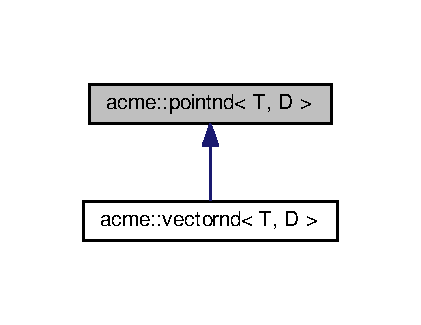
\includegraphics[width=202pt]{d2/d2b/classacme_1_1pointnd__inherit__graph}
\end{center}
\end{figure}
\subsection*{Public Member Functions}
\begin{DoxyCompactItemize}
\item 
\mbox{\Hypertarget{classacme_1_1pointnd_a284231947c22b4796ab74878d257160e}\label{classacme_1_1pointnd_a284231947c22b4796ab74878d257160e}} 
\hyperlink{classacme_1_1pointnd_a284231947c22b4796ab74878d257160e}{pointnd} ()
\begin{DoxyCompactList}\small\item\em Class constructor. \end{DoxyCompactList}\item 
\hyperlink{classacme_1_1pointnd_aeabd8c2c9028247e3f92362755aa9806}{pointnd} (const T \&value0)
\begin{DoxyCompactList}\small\item\em Class constructor. \end{DoxyCompactList}\item 
\hyperlink{classacme_1_1pointnd_a44a24023bae0c265fa59db90003ff916}{pointnd} (const T \&value0, const T \&value1)
\begin{DoxyCompactList}\small\item\em Class constructor. \end{DoxyCompactList}\item 
\hyperlink{classacme_1_1pointnd_aac9ecea0a96f3b6d9a9e3b39066785d2}{pointnd} (const T \&value0, const T \&value1, const T \&value2)
\begin{DoxyCompactList}\small\item\em Class constructor. \end{DoxyCompactList}\item 
\hyperlink{classacme_1_1pointnd_aec3e1e45adcfc4e6094fcb46c454708a}{pointnd} (const T \&value0, const T \&value1, const T \&value2, const T \&value3)
\begin{DoxyCompactList}\small\item\em Class constructor. \end{DoxyCompactList}\item 
\hyperlink{classacme_1_1pointnd_a70c00125fb976462a993f2edfc06870d}{pointnd} (const \hyperlink{classacme_1_1pointnd}{pointnd}$<$ T, D $>$ \&\hyperlink{classacme_1_1point}{point})
\begin{DoxyCompactList}\small\item\em Class constructor. \end{DoxyCompactList}\item 
\hyperlink{classacme_1_1pointnd_a79fb8863dcfbca679747b145dae7f0d8}{pointnd} (const \hyperlink{classacme_1_1point2d}{point2d}$<$ T $>$ \&\hyperlink{classacme_1_1point}{point})
\begin{DoxyCompactList}\small\item\em Class constructor. \end{DoxyCompactList}\item 
\hyperlink{classacme_1_1pointnd_a7f0e5434f15d3f5d2f97ba3d1dbcec6e}{pointnd} (const \hyperlink{classacme_1_1point3d}{point3d}$<$ T $>$ \&\hyperlink{classacme_1_1point}{point})
\begin{DoxyCompactList}\small\item\em Class constructor. \end{DoxyCompactList}\item 
\mbox{\Hypertarget{classacme_1_1pointnd_a07c983b5a2d653304d6ed0294b8f55b5}\label{classacme_1_1pointnd_a07c983b5a2d653304d6ed0294b8f55b5}} 
\hyperlink{classacme_1_1pointnd_a07c983b5a2d653304d6ed0294b8f55b5}{$\sim$pointnd} ()
\begin{DoxyCompactList}\small\item\em Class destructor. \end{DoxyCompactList}\item 
\mbox{\Hypertarget{classacme_1_1pointnd_a2d0b84e609dc1ad5cbbe631c5bb5791f}\label{classacme_1_1pointnd_a2d0b84e609dc1ad5cbbe631c5bb5791f}} 
void \hyperlink{classacme_1_1pointnd_a2d0b84e609dc1ad5cbbe631c5bb5791f}{clear} ()
\begin{DoxyCompactList}\small\item\em Clear vector data. \end{DoxyCompactList}\item 
\hyperlink{classacme_1_1pointnd}{pointnd}$<$ T, D $>$ \& \hyperlink{classacme_1_1pointnd_ad4196b71eee0aef40771f864c23e9f13}{operator=} (const \hyperlink{classacme_1_1pointnd}{pointnd}$<$ T, D $>$ \&\hyperlink{classacme_1_1point}{point})
\begin{DoxyCompactList}\small\item\em Equality operator. \end{DoxyCompactList}\item 
\hyperlink{classacme_1_1pointnd}{pointnd}$<$ T, D $>$ \& \hyperlink{classacme_1_1pointnd_a8a548f2642065ade8e0e8666aafc448a}{operator=} (const \hyperlink{classacme_1_1point2d}{point2d}$<$ T $>$ \&\hyperlink{classacme_1_1point}{point})
\begin{DoxyCompactList}\small\item\em Equality operator. \end{DoxyCompactList}\item 
\hyperlink{classacme_1_1pointnd}{pointnd}$<$ T, D $>$ \& \hyperlink{classacme_1_1pointnd_a90082456348fdb8303c5cf9d31abe847}{operator=} (const \hyperlink{classacme_1_1point3d}{point3d}$<$ T $>$ \&\hyperlink{classacme_1_1point}{point})
\begin{DoxyCompactList}\small\item\em Equality operator. \end{DoxyCompactList}\item 
T \& \hyperlink{classacme_1_1pointnd_a35b0691673728d98d455c007612d6b91}{operator\mbox{[}$\,$\mbox{]}} (const std\+::size\+\_\+t \&index)
\begin{DoxyCompactList}\small\item\em Indexing operator. \end{DoxyCompactList}\item 
const T \& \hyperlink{classacme_1_1pointnd_a565e9ed195c8f8dadc570a029a3deb94}{operator\mbox{[}$\,$\mbox{]}} (const std\+::size\+\_\+t \&index) const
\begin{DoxyCompactList}\small\item\em Indexing operator. \end{DoxyCompactList}\end{DoxyCompactItemize}
\subsection*{Protected Attributes}
\begin{DoxyCompactItemize}
\item 
\mbox{\Hypertarget{classacme_1_1pointnd_a13b19080ed617e2a9c5d6058f07d4f4b}\label{classacme_1_1pointnd_a13b19080ed617e2a9c5d6058f07d4f4b}} 
Eigen\+::\+Matrix$<$ T, D, 1 $>$ {\bfseries data}
\end{DoxyCompactItemize}


\subsection{Detailed Description}
\subsubsection*{template$<$typename T, std\+::size\+\_\+t D$>$\newline
class acme\+::pointnd$<$ T, D $>$}

N-\/dimensional point class container. 

\subsection{Constructor \& Destructor Documentation}
\mbox{\Hypertarget{classacme_1_1pointnd_aeabd8c2c9028247e3f92362755aa9806}\label{classacme_1_1pointnd_aeabd8c2c9028247e3f92362755aa9806}} 
\index{acme\+::pointnd@{acme\+::pointnd}!pointnd@{pointnd}}
\index{pointnd@{pointnd}!acme\+::pointnd@{acme\+::pointnd}}
\subsubsection{\texorpdfstring{pointnd()}{pointnd()}\hspace{0.1cm}{\footnotesize\ttfamily [1/7]}}
{\footnotesize\ttfamily template$<$typename T, std\+::size\+\_\+t D$>$ \\
\hyperlink{classacme_1_1pointnd}{acme\+::pointnd}$<$ T, D $>$\+::\hyperlink{classacme_1_1pointnd}{pointnd} (\begin{DoxyParamCaption}\item[{const T \&}]{value0 }\end{DoxyParamCaption})\hspace{0.3cm}{\ttfamily [inline]}}



Class constructor. 


\begin{DoxyParams}{Parameters}
{\em value0} & Input value 0 \\
\hline
\end{DoxyParams}
\mbox{\Hypertarget{classacme_1_1pointnd_a44a24023bae0c265fa59db90003ff916}\label{classacme_1_1pointnd_a44a24023bae0c265fa59db90003ff916}} 
\index{acme\+::pointnd@{acme\+::pointnd}!pointnd@{pointnd}}
\index{pointnd@{pointnd}!acme\+::pointnd@{acme\+::pointnd}}
\subsubsection{\texorpdfstring{pointnd()}{pointnd()}\hspace{0.1cm}{\footnotesize\ttfamily [2/7]}}
{\footnotesize\ttfamily template$<$typename T, std\+::size\+\_\+t D$>$ \\
\hyperlink{classacme_1_1pointnd}{acme\+::pointnd}$<$ T, D $>$\+::\hyperlink{classacme_1_1pointnd}{pointnd} (\begin{DoxyParamCaption}\item[{const T \&}]{value0,  }\item[{const T \&}]{value1 }\end{DoxyParamCaption})\hspace{0.3cm}{\ttfamily [inline]}}



Class constructor. 


\begin{DoxyParams}{Parameters}
{\em value0} & Input value 0 \\
\hline
{\em value1} & Input value 1 \\
\hline
\end{DoxyParams}
\mbox{\Hypertarget{classacme_1_1pointnd_aac9ecea0a96f3b6d9a9e3b39066785d2}\label{classacme_1_1pointnd_aac9ecea0a96f3b6d9a9e3b39066785d2}} 
\index{acme\+::pointnd@{acme\+::pointnd}!pointnd@{pointnd}}
\index{pointnd@{pointnd}!acme\+::pointnd@{acme\+::pointnd}}
\subsubsection{\texorpdfstring{pointnd()}{pointnd()}\hspace{0.1cm}{\footnotesize\ttfamily [3/7]}}
{\footnotesize\ttfamily template$<$typename T, std\+::size\+\_\+t D$>$ \\
\hyperlink{classacme_1_1pointnd}{acme\+::pointnd}$<$ T, D $>$\+::\hyperlink{classacme_1_1pointnd}{pointnd} (\begin{DoxyParamCaption}\item[{const T \&}]{value0,  }\item[{const T \&}]{value1,  }\item[{const T \&}]{value2 }\end{DoxyParamCaption})\hspace{0.3cm}{\ttfamily [inline]}}



Class constructor. 


\begin{DoxyParams}{Parameters}
{\em value0} & Input value 0 \\
\hline
{\em value1} & Input value 1 \\
\hline
{\em value2} & Input value 2 \\
\hline
\end{DoxyParams}
\mbox{\Hypertarget{classacme_1_1pointnd_aec3e1e45adcfc4e6094fcb46c454708a}\label{classacme_1_1pointnd_aec3e1e45adcfc4e6094fcb46c454708a}} 
\index{acme\+::pointnd@{acme\+::pointnd}!pointnd@{pointnd}}
\index{pointnd@{pointnd}!acme\+::pointnd@{acme\+::pointnd}}
\subsubsection{\texorpdfstring{pointnd()}{pointnd()}\hspace{0.1cm}{\footnotesize\ttfamily [4/7]}}
{\footnotesize\ttfamily template$<$typename T, std\+::size\+\_\+t D$>$ \\
\hyperlink{classacme_1_1pointnd}{acme\+::pointnd}$<$ T, D $>$\+::\hyperlink{classacme_1_1pointnd}{pointnd} (\begin{DoxyParamCaption}\item[{const T \&}]{value0,  }\item[{const T \&}]{value1,  }\item[{const T \&}]{value2,  }\item[{const T \&}]{value3 }\end{DoxyParamCaption})\hspace{0.3cm}{\ttfamily [inline]}}



Class constructor. 


\begin{DoxyParams}{Parameters}
{\em value0} & Input value 0 \\
\hline
{\em value1} & Input value 1 \\
\hline
{\em value2} & Input value 2 \\
\hline
{\em value3} & Input value 3 \\
\hline
\end{DoxyParams}
\mbox{\Hypertarget{classacme_1_1pointnd_a70c00125fb976462a993f2edfc06870d}\label{classacme_1_1pointnd_a70c00125fb976462a993f2edfc06870d}} 
\index{acme\+::pointnd@{acme\+::pointnd}!pointnd@{pointnd}}
\index{pointnd@{pointnd}!acme\+::pointnd@{acme\+::pointnd}}
\subsubsection{\texorpdfstring{pointnd()}{pointnd()}\hspace{0.1cm}{\footnotesize\ttfamily [5/7]}}
{\footnotesize\ttfamily template$<$typename T, std\+::size\+\_\+t D$>$ \\
\hyperlink{classacme_1_1pointnd}{acme\+::pointnd}$<$ T, D $>$\+::\hyperlink{classacme_1_1pointnd}{pointnd} (\begin{DoxyParamCaption}\item[{const \hyperlink{classacme_1_1pointnd}{pointnd}$<$ T, D $>$ \&}]{point }\end{DoxyParamCaption})\hspace{0.3cm}{\ttfamily [inline]}}



Class constructor. 


\begin{DoxyParams}{Parameters}
{\em point} & Input N-\/dimensional point \\
\hline
\end{DoxyParams}
\mbox{\Hypertarget{classacme_1_1pointnd_a79fb8863dcfbca679747b145dae7f0d8}\label{classacme_1_1pointnd_a79fb8863dcfbca679747b145dae7f0d8}} 
\index{acme\+::pointnd@{acme\+::pointnd}!pointnd@{pointnd}}
\index{pointnd@{pointnd}!acme\+::pointnd@{acme\+::pointnd}}
\subsubsection{\texorpdfstring{pointnd()}{pointnd()}\hspace{0.1cm}{\footnotesize\ttfamily [6/7]}}
{\footnotesize\ttfamily template$<$typename T, std\+::size\+\_\+t D$>$ \\
\hyperlink{classacme_1_1pointnd}{acme\+::pointnd}$<$ T, D $>$\+::\hyperlink{classacme_1_1pointnd}{pointnd} (\begin{DoxyParamCaption}\item[{const \hyperlink{classacme_1_1point2d}{point2d}$<$ T $>$ \&}]{point }\end{DoxyParamCaption})\hspace{0.3cm}{\ttfamily [inline]}}



Class constructor. 


\begin{DoxyParams}{Parameters}
{\em point} & Input 2-\/dimensional point \\
\hline
\end{DoxyParams}
\mbox{\Hypertarget{classacme_1_1pointnd_a7f0e5434f15d3f5d2f97ba3d1dbcec6e}\label{classacme_1_1pointnd_a7f0e5434f15d3f5d2f97ba3d1dbcec6e}} 
\index{acme\+::pointnd@{acme\+::pointnd}!pointnd@{pointnd}}
\index{pointnd@{pointnd}!acme\+::pointnd@{acme\+::pointnd}}
\subsubsection{\texorpdfstring{pointnd()}{pointnd()}\hspace{0.1cm}{\footnotesize\ttfamily [7/7]}}
{\footnotesize\ttfamily template$<$typename T, std\+::size\+\_\+t D$>$ \\
\hyperlink{classacme_1_1pointnd}{acme\+::pointnd}$<$ T, D $>$\+::\hyperlink{classacme_1_1pointnd}{pointnd} (\begin{DoxyParamCaption}\item[{const \hyperlink{classacme_1_1point3d}{point3d}$<$ T $>$ \&}]{point }\end{DoxyParamCaption})\hspace{0.3cm}{\ttfamily [inline]}}



Class constructor. 


\begin{DoxyParams}{Parameters}
{\em point} & Input 3-\/dimensional point \\
\hline
\end{DoxyParams}


\subsection{Member Function Documentation}
\mbox{\Hypertarget{classacme_1_1pointnd_ad4196b71eee0aef40771f864c23e9f13}\label{classacme_1_1pointnd_ad4196b71eee0aef40771f864c23e9f13}} 
\index{acme\+::pointnd@{acme\+::pointnd}!operator=@{operator=}}
\index{operator=@{operator=}!acme\+::pointnd@{acme\+::pointnd}}
\subsubsection{\texorpdfstring{operator=()}{operator=()}\hspace{0.1cm}{\footnotesize\ttfamily [1/3]}}
{\footnotesize\ttfamily template$<$typename T, std\+::size\+\_\+t D$>$ \\
\hyperlink{classacme_1_1pointnd}{pointnd}$<$T, D$>$\& \hyperlink{classacme_1_1pointnd}{acme\+::pointnd}$<$ T, D $>$\+::operator= (\begin{DoxyParamCaption}\item[{const \hyperlink{classacme_1_1pointnd}{pointnd}$<$ T, D $>$ \&}]{point }\end{DoxyParamCaption})\hspace{0.3cm}{\ttfamily [inline]}}



Equality operator. 


\begin{DoxyParams}{Parameters}
{\em point} & Input N-\/dimensional point \\
\hline
\end{DoxyParams}
\mbox{\Hypertarget{classacme_1_1pointnd_a8a548f2642065ade8e0e8666aafc448a}\label{classacme_1_1pointnd_a8a548f2642065ade8e0e8666aafc448a}} 
\index{acme\+::pointnd@{acme\+::pointnd}!operator=@{operator=}}
\index{operator=@{operator=}!acme\+::pointnd@{acme\+::pointnd}}
\subsubsection{\texorpdfstring{operator=()}{operator=()}\hspace{0.1cm}{\footnotesize\ttfamily [2/3]}}
{\footnotesize\ttfamily template$<$typename T, std\+::size\+\_\+t D$>$ \\
\hyperlink{classacme_1_1pointnd}{pointnd}$<$T, D$>$\& \hyperlink{classacme_1_1pointnd}{acme\+::pointnd}$<$ T, D $>$\+::operator= (\begin{DoxyParamCaption}\item[{const \hyperlink{classacme_1_1point2d}{point2d}$<$ T $>$ \&}]{point }\end{DoxyParamCaption})\hspace{0.3cm}{\ttfamily [inline]}}



Equality operator. 


\begin{DoxyParams}{Parameters}
{\em point} & Input 2-\/dimensional point \\
\hline
\end{DoxyParams}
\mbox{\Hypertarget{classacme_1_1pointnd_a90082456348fdb8303c5cf9d31abe847}\label{classacme_1_1pointnd_a90082456348fdb8303c5cf9d31abe847}} 
\index{acme\+::pointnd@{acme\+::pointnd}!operator=@{operator=}}
\index{operator=@{operator=}!acme\+::pointnd@{acme\+::pointnd}}
\subsubsection{\texorpdfstring{operator=()}{operator=()}\hspace{0.1cm}{\footnotesize\ttfamily [3/3]}}
{\footnotesize\ttfamily template$<$typename T, std\+::size\+\_\+t D$>$ \\
\hyperlink{classacme_1_1pointnd}{pointnd}$<$T, D$>$\& \hyperlink{classacme_1_1pointnd}{acme\+::pointnd}$<$ T, D $>$\+::operator= (\begin{DoxyParamCaption}\item[{const \hyperlink{classacme_1_1point3d}{point3d}$<$ T $>$ \&}]{point }\end{DoxyParamCaption})\hspace{0.3cm}{\ttfamily [inline]}}



Equality operator. 


\begin{DoxyParams}{Parameters}
{\em point} & Input 3-\/dimensional point \\
\hline
\end{DoxyParams}
\mbox{\Hypertarget{classacme_1_1pointnd_a35b0691673728d98d455c007612d6b91}\label{classacme_1_1pointnd_a35b0691673728d98d455c007612d6b91}} 
\index{acme\+::pointnd@{acme\+::pointnd}!operator\mbox{[}\mbox{]}@{operator[]}}
\index{operator\mbox{[}\mbox{]}@{operator[]}!acme\+::pointnd@{acme\+::pointnd}}
\subsubsection{\texorpdfstring{operator[]()}{operator[]()}\hspace{0.1cm}{\footnotesize\ttfamily [1/2]}}
{\footnotesize\ttfamily template$<$typename T, std\+::size\+\_\+t D$>$ \\
T\& \hyperlink{classacme_1_1pointnd}{acme\+::pointnd}$<$ T, D $>$\+::operator\mbox{[}$\,$\mbox{]} (\begin{DoxyParamCaption}\item[{const std\+::size\+\_\+t \&}]{index }\end{DoxyParamCaption})\hspace{0.3cm}{\ttfamily [inline]}}



Indexing operator. 


\begin{DoxyParams}{Parameters}
{\em index} & Input index \\
\hline
\end{DoxyParams}
\mbox{\Hypertarget{classacme_1_1pointnd_a565e9ed195c8f8dadc570a029a3deb94}\label{classacme_1_1pointnd_a565e9ed195c8f8dadc570a029a3deb94}} 
\index{acme\+::pointnd@{acme\+::pointnd}!operator\mbox{[}\mbox{]}@{operator[]}}
\index{operator\mbox{[}\mbox{]}@{operator[]}!acme\+::pointnd@{acme\+::pointnd}}
\subsubsection{\texorpdfstring{operator[]()}{operator[]()}\hspace{0.1cm}{\footnotesize\ttfamily [2/2]}}
{\footnotesize\ttfamily template$<$typename T, std\+::size\+\_\+t D$>$ \\
const T\& \hyperlink{classacme_1_1pointnd}{acme\+::pointnd}$<$ T, D $>$\+::operator\mbox{[}$\,$\mbox{]} (\begin{DoxyParamCaption}\item[{const std\+::size\+\_\+t \&}]{index }\end{DoxyParamCaption}) const\hspace{0.3cm}{\ttfamily [inline]}}



Indexing operator. 


\begin{DoxyParams}{Parameters}
{\em index} & Input index \\
\hline
\end{DoxyParams}


The documentation for this class was generated from the following file\+:\begin{DoxyCompactItemize}
\item 
src/acme\+\_\+point.\+hh\end{DoxyCompactItemize}

\hypertarget{classacme_1_1segment2d}{}\section{acme\+:\+:segment2d$<$ T $>$ Class Template Reference}
\label{classacme_1_1segment2d}\index{acme\+::segment2d$<$ T $>$@{acme\+::segment2d$<$ T $>$}}


Inheritance diagram for acme\+:\+:segment2d$<$ T $>$\+:
\nopagebreak
\begin{figure}[H]
\begin{center}
\leavevmode
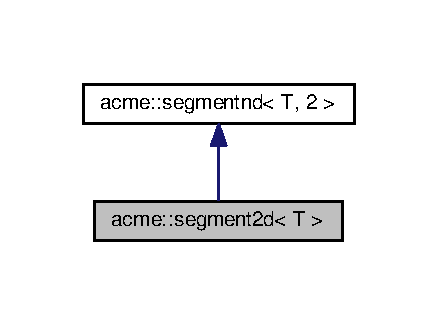
\includegraphics[width=210pt]{d6/dbd/classacme_1_1segment2d__inherit__graph}
\end{center}
\end{figure}


Collaboration diagram for acme\+:\+:segment2d$<$ T $>$\+:
\nopagebreak
\begin{figure}[H]
\begin{center}
\leavevmode
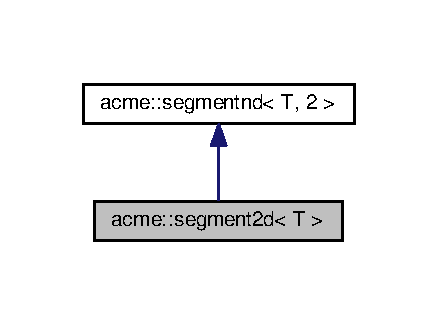
\includegraphics[width=210pt]{de/df2/classacme_1_1segment2d__coll__graph}
\end{center}
\end{figure}
\subsection*{Public Member Functions}
\begin{DoxyCompactItemize}
\item 
\mbox{\Hypertarget{classacme_1_1segmentnd_a8635bff51cdc526e812cf1d49f74054b}\label{classacme_1_1segmentnd_a8635bff51cdc526e812cf1d49f74054b}} 
\hyperlink{classacme_1_1pointnd}{pointnd}$<$ T, D $>$ \& {\bfseries operator\mbox{[}$\,$\mbox{]}} (const std\+::size\+\_\+t \&index)
\item 
\mbox{\Hypertarget{classacme_1_1segmentnd_a1b40e0a378245df5db64af1e4ec262ab}\label{classacme_1_1segmentnd_a1b40e0a378245df5db64af1e4ec262ab}} 
const \hyperlink{classacme_1_1pointnd}{pointnd}$<$ T, D $>$ \& {\bfseries operator\mbox{[}$\,$\mbox{]}} (const std\+::size\+\_\+t \&index) const
\item 
\mbox{\Hypertarget{classacme_1_1segmentnd_a844a5fbdb6cb3fc4a8bfcd98039e235e}\label{classacme_1_1segmentnd_a844a5fbdb6cb3fc4a8bfcd98039e235e}} 
std\+::size\+\_\+t {\bfseries size} ()
\end{DoxyCompactItemize}


The documentation for this class was generated from the following file\+:\begin{DoxyCompactItemize}
\item 
src/acme\+\_\+segment.\+hh\end{DoxyCompactItemize}

\hypertarget{classacme_1_1segment3d}{}\section{acme\+:\+:segment3d$<$ T $>$ Class Template Reference}
\label{classacme_1_1segment3d}\index{acme\+::segment3d$<$ T $>$@{acme\+::segment3d$<$ T $>$}}


Inheritance diagram for acme\+:\+:segment3d$<$ T $>$\+:
\nopagebreak
\begin{figure}[H]
\begin{center}
\leavevmode
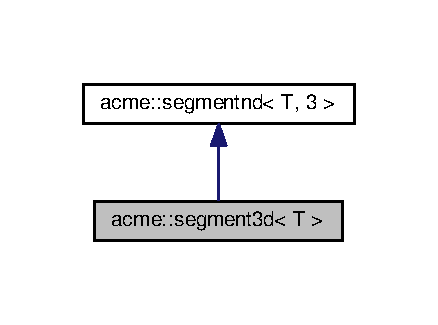
\includegraphics[width=210pt]{dd/d7f/classacme_1_1segment3d__inherit__graph}
\end{center}
\end{figure}


Collaboration diagram for acme\+:\+:segment3d$<$ T $>$\+:
\nopagebreak
\begin{figure}[H]
\begin{center}
\leavevmode
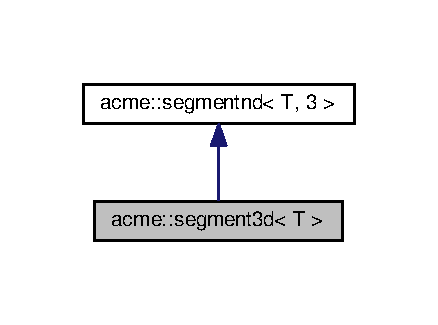
\includegraphics[width=210pt]{db/d30/classacme_1_1segment3d__coll__graph}
\end{center}
\end{figure}
\subsection*{Public Member Functions}
\begin{DoxyCompactItemize}
\item 
\mbox{\Hypertarget{classacme_1_1segmentnd_a8635bff51cdc526e812cf1d49f74054b}\label{classacme_1_1segmentnd_a8635bff51cdc526e812cf1d49f74054b}} 
\hyperlink{classacme_1_1pointnd}{pointnd}$<$ T, D $>$ \& {\bfseries operator\mbox{[}$\,$\mbox{]}} (const std\+::size\+\_\+t \&index)
\item 
\mbox{\Hypertarget{classacme_1_1segmentnd_a1b40e0a378245df5db64af1e4ec262ab}\label{classacme_1_1segmentnd_a1b40e0a378245df5db64af1e4ec262ab}} 
const \hyperlink{classacme_1_1pointnd}{pointnd}$<$ T, D $>$ \& {\bfseries operator\mbox{[}$\,$\mbox{]}} (const std\+::size\+\_\+t \&index) const
\item 
\mbox{\Hypertarget{classacme_1_1segmentnd_a844a5fbdb6cb3fc4a8bfcd98039e235e}\label{classacme_1_1segmentnd_a844a5fbdb6cb3fc4a8bfcd98039e235e}} 
std\+::size\+\_\+t {\bfseries size} ()
\end{DoxyCompactItemize}


The documentation for this class was generated from the following file\+:\begin{DoxyCompactItemize}
\item 
src/acme\+\_\+segment.\+hh\end{DoxyCompactItemize}

\hypertarget{classacme_1_1segmentnd}{}\section{acme\+:\+:segmentnd$<$ T, D $>$ Class Template Reference}
\label{classacme_1_1segmentnd}\index{acme\+::segmentnd$<$ T, D $>$@{acme\+::segmentnd$<$ T, D $>$}}
\subsection*{Public Member Functions}
\begin{DoxyCompactItemize}
\item 
\mbox{\Hypertarget{classacme_1_1segmentnd_abec50f4ebea3cdb91588b2b05d5f5f49}\label{classacme_1_1segmentnd_abec50f4ebea3cdb91588b2b05d5f5f49}} 
\hyperlink{classacme_1_1segmentnd_abec50f4ebea3cdb91588b2b05d5f5f49}{segmentnd} ()
\begin{DoxyCompactList}\small\item\em Class constructor. \end{DoxyCompactList}\item 
\mbox{\Hypertarget{classacme_1_1segmentnd_abb83fe93ca44db6d03031e130f27981d}\label{classacme_1_1segmentnd_abb83fe93ca44db6d03031e130f27981d}} 
\hyperlink{classacme_1_1segmentnd_abb83fe93ca44db6d03031e130f27981d}{segmentnd} (const T \&x0, const T \&y0, const T \&x1, const T \&y1)
\begin{DoxyCompactList}\small\item\em Class constructor. \end{DoxyCompactList}\item 
\mbox{\Hypertarget{classacme_1_1segmentnd_ad8752db6cd23acaac5f3d906fa9105b8}\label{classacme_1_1segmentnd_ad8752db6cd23acaac5f3d906fa9105b8}} 
\hyperlink{classacme_1_1segmentnd_ad8752db6cd23acaac5f3d906fa9105b8}{segmentnd} (const T \&x0, const T \&y0, const T \&z0, const T \&x1, const T \&y1, const T \&z1)
\begin{DoxyCompactList}\small\item\em Class constructor. \end{DoxyCompactList}\item 
\hyperlink{classacme_1_1segmentnd_ad0838ae4990ff412110d11524a416b3f}{segmentnd} (const \hyperlink{classacme_1_1point2d}{point2d}$<$ T $>$ \&point0, const \hyperlink{classacme_1_1point2d}{point2d}$<$ T $>$ \&point1)
\begin{DoxyCompactList}\small\item\em Class constructor. \end{DoxyCompactList}\item 
\hyperlink{classacme_1_1segmentnd_a806b9abc096ae1dd9e94c88b3a8f0e97}{segmentnd} (const \hyperlink{classacme_1_1point3d}{point3d}$<$ T $>$ \&point0, const \hyperlink{classacme_1_1point3d}{point3d}$<$ T $>$ \&point1)
\begin{DoxyCompactList}\small\item\em Class constructor. \end{DoxyCompactList}\item 
\hyperlink{classacme_1_1segmentnd_a0f6c38e8fe244f629a0f34a3451f8ead}{segmentnd} (const \hyperlink{classacme_1_1pointnd}{pointnd}$<$ T, D $>$ \&point0, const \hyperlink{classacme_1_1pointnd}{pointnd}$<$ T, D $>$ \&point1)
\begin{DoxyCompactList}\small\item\em Class constructor. \end{DoxyCompactList}\item 
\hyperlink{classacme_1_1segmentnd_a4afa0be2c691e1c8a7239f547879538f}{segmentnd} (const \hyperlink{classacme_1_1segment2d}{segment2d}$<$ T $>$ \&segment)
\begin{DoxyCompactList}\small\item\em Class constructor. \end{DoxyCompactList}\item 
\mbox{\Hypertarget{classacme_1_1segmentnd_a128c5e8c6b324590001b44bbd1df376d}\label{classacme_1_1segmentnd_a128c5e8c6b324590001b44bbd1df376d}} 
\hyperlink{classacme_1_1segmentnd_a128c5e8c6b324590001b44bbd1df376d}{$\sim$segmentnd} ()
\begin{DoxyCompactList}\small\item\em Class destructor. \end{DoxyCompactList}\item 
\mbox{\Hypertarget{classacme_1_1segmentnd_a8635bff51cdc526e812cf1d49f74054b}\label{classacme_1_1segmentnd_a8635bff51cdc526e812cf1d49f74054b}} 
\hyperlink{classacme_1_1pointnd}{pointnd}$<$ T, D $>$ \& {\bfseries operator\mbox{[}$\,$\mbox{]}} (const std\+::size\+\_\+t \&index)
\item 
\mbox{\Hypertarget{classacme_1_1segmentnd_a1b40e0a378245df5db64af1e4ec262ab}\label{classacme_1_1segmentnd_a1b40e0a378245df5db64af1e4ec262ab}} 
const \hyperlink{classacme_1_1pointnd}{pointnd}$<$ T, D $>$ \& {\bfseries operator\mbox{[}$\,$\mbox{]}} (const std\+::size\+\_\+t \&index) const
\item 
\mbox{\Hypertarget{classacme_1_1segmentnd_a844a5fbdb6cb3fc4a8bfcd98039e235e}\label{classacme_1_1segmentnd_a844a5fbdb6cb3fc4a8bfcd98039e235e}} 
std\+::size\+\_\+t {\bfseries size} ()
\end{DoxyCompactItemize}


\subsection{Constructor \& Destructor Documentation}
\mbox{\Hypertarget{classacme_1_1segmentnd_ad0838ae4990ff412110d11524a416b3f}\label{classacme_1_1segmentnd_ad0838ae4990ff412110d11524a416b3f}} 
\index{acme\+::segmentnd@{acme\+::segmentnd}!segmentnd@{segmentnd}}
\index{segmentnd@{segmentnd}!acme\+::segmentnd@{acme\+::segmentnd}}
\subsubsection{\texorpdfstring{segmentnd()}{segmentnd()}\hspace{0.1cm}{\footnotesize\ttfamily [1/4]}}
{\footnotesize\ttfamily template$<$typename T, std\+::size\+\_\+t D$>$ \\
\hyperlink{classacme_1_1segmentnd}{acme\+::segmentnd}$<$ T, D $>$\+::\hyperlink{classacme_1_1segmentnd}{segmentnd} (\begin{DoxyParamCaption}\item[{const \hyperlink{classacme_1_1point2d}{point2d}$<$ T $>$ \&}]{point0,  }\item[{const \hyperlink{classacme_1_1point2d}{point2d}$<$ T $>$ \&}]{point1 }\end{DoxyParamCaption})\hspace{0.3cm}{\ttfamily [inline]}}



Class constructor. 


\begin{DoxyParams}{Parameters}
{\em point0} & Input 2-\/dimensional point \\
\hline
{\em point1} & Input 2-\/dimensional point \\
\hline
\end{DoxyParams}
\mbox{\Hypertarget{classacme_1_1segmentnd_a806b9abc096ae1dd9e94c88b3a8f0e97}\label{classacme_1_1segmentnd_a806b9abc096ae1dd9e94c88b3a8f0e97}} 
\index{acme\+::segmentnd@{acme\+::segmentnd}!segmentnd@{segmentnd}}
\index{segmentnd@{segmentnd}!acme\+::segmentnd@{acme\+::segmentnd}}
\subsubsection{\texorpdfstring{segmentnd()}{segmentnd()}\hspace{0.1cm}{\footnotesize\ttfamily [2/4]}}
{\footnotesize\ttfamily template$<$typename T, std\+::size\+\_\+t D$>$ \\
\hyperlink{classacme_1_1segmentnd}{acme\+::segmentnd}$<$ T, D $>$\+::\hyperlink{classacme_1_1segmentnd}{segmentnd} (\begin{DoxyParamCaption}\item[{const \hyperlink{classacme_1_1point3d}{point3d}$<$ T $>$ \&}]{point0,  }\item[{const \hyperlink{classacme_1_1point3d}{point3d}$<$ T $>$ \&}]{point1 }\end{DoxyParamCaption})\hspace{0.3cm}{\ttfamily [inline]}}



Class constructor. 


\begin{DoxyParams}{Parameters}
{\em point0} & Input 3-\/dimensional point \\
\hline
{\em point1} & Input 3-\/dimensional point \\
\hline
\end{DoxyParams}
\mbox{\Hypertarget{classacme_1_1segmentnd_a0f6c38e8fe244f629a0f34a3451f8ead}\label{classacme_1_1segmentnd_a0f6c38e8fe244f629a0f34a3451f8ead}} 
\index{acme\+::segmentnd@{acme\+::segmentnd}!segmentnd@{segmentnd}}
\index{segmentnd@{segmentnd}!acme\+::segmentnd@{acme\+::segmentnd}}
\subsubsection{\texorpdfstring{segmentnd()}{segmentnd()}\hspace{0.1cm}{\footnotesize\ttfamily [3/4]}}
{\footnotesize\ttfamily template$<$typename T, std\+::size\+\_\+t D$>$ \\
\hyperlink{classacme_1_1segmentnd}{acme\+::segmentnd}$<$ T, D $>$\+::\hyperlink{classacme_1_1segmentnd}{segmentnd} (\begin{DoxyParamCaption}\item[{const \hyperlink{classacme_1_1pointnd}{pointnd}$<$ T, D $>$ \&}]{point0,  }\item[{const \hyperlink{classacme_1_1pointnd}{pointnd}$<$ T, D $>$ \&}]{point1 }\end{DoxyParamCaption})\hspace{0.3cm}{\ttfamily [inline]}}



Class constructor. 


\begin{DoxyParams}{Parameters}
{\em point0} & Input N-\/dimensional point \\
\hline
{\em point1} & Input N-\/dimensional point \\
\hline
\end{DoxyParams}
\mbox{\Hypertarget{classacme_1_1segmentnd_a4afa0be2c691e1c8a7239f547879538f}\label{classacme_1_1segmentnd_a4afa0be2c691e1c8a7239f547879538f}} 
\index{acme\+::segmentnd@{acme\+::segmentnd}!segmentnd@{segmentnd}}
\index{segmentnd@{segmentnd}!acme\+::segmentnd@{acme\+::segmentnd}}
\subsubsection{\texorpdfstring{segmentnd()}{segmentnd()}\hspace{0.1cm}{\footnotesize\ttfamily [4/4]}}
{\footnotesize\ttfamily template$<$typename T, std\+::size\+\_\+t D$>$ \\
\hyperlink{classacme_1_1segmentnd}{acme\+::segmentnd}$<$ T, D $>$\+::\hyperlink{classacme_1_1segmentnd}{segmentnd} (\begin{DoxyParamCaption}\item[{const \hyperlink{classacme_1_1segment2d}{segment2d}$<$ T $>$ \&}]{segment }\end{DoxyParamCaption})\hspace{0.3cm}{\ttfamily [inline]}}



Class constructor. 


\begin{DoxyParams}{Parameters}
{\em segment} & Input 2-\/dimensional segment \\
\hline
\end{DoxyParams}


The documentation for this class was generated from the following file\+:\begin{DoxyCompactItemize}
\item 
src/acme\+\_\+segment.\+hh\end{DoxyCompactItemize}

\hypertarget{class_tic_toc}{}\section{Tic\+Toc Class Reference}
\label{class_tic_toc}\index{Tic\+Toc@{Tic\+Toc}}
\subsection*{Public Member Functions}
\begin{DoxyCompactItemize}
\item 
\mbox{\Hypertarget{class_tic_toc_a5d76802851d3cbc366b4ccccb7257e2e}\label{class_tic_toc_a5d76802851d3cbc366b4ccccb7257e2e}} 
void {\bfseries tic} ()
\item 
\mbox{\Hypertarget{class_tic_toc_a911de3386cba55c573850588f0080007}\label{class_tic_toc_a911de3386cba55c573850588f0080007}} 
void {\bfseries toc} ()
\item 
\mbox{\Hypertarget{class_tic_toc_acf23c55f595a03da92bda44a2127143d}\label{class_tic_toc_acf23c55f595a03da92bda44a2127143d}} 
real\+\_\+type {\bfseries elapsed\+\_\+s} () const
\item 
\mbox{\Hypertarget{class_tic_toc_a2cf72ce8e4452dca5c05e38002281312}\label{class_tic_toc_a2cf72ce8e4452dca5c05e38002281312}} 
real\+\_\+type {\bfseries elapsed\+\_\+ms} () const
\end{DoxyCompactItemize}


The documentation for this class was generated from the following file\+:\begin{DoxyCompactItemize}
\item 
src/Tic\+Toc.\+hh\end{DoxyCompactItemize}

\hypertarget{classacme_1_1triangle}{}\section{acme\+:\+:triangle$<$ T, D $>$ Class Template Reference}
\label{classacme_1_1triangle}\index{acme\+::triangle$<$ T, D $>$@{acme\+::triangle$<$ T, D $>$}}


ND triangle class container.  




{\ttfamily \#include $<$acme\+\_\+triangle.\+hh$>$}

\subsection*{Public Member Functions}
\begin{DoxyCompactItemize}
\item 
\mbox{\Hypertarget{classacme_1_1triangle_ab848f5a31e2f426704277802cae23e20}\label{classacme_1_1triangle_ab848f5a31e2f426704277802cae23e20}} 
\hyperlink{classacme_1_1triangle_ab848f5a31e2f426704277802cae23e20}{triangle} (const \hyperlink{classacme_1_1triangle}{triangle}$<$ T, D $>$ \&)=default
\begin{DoxyCompactList}\small\item\em Copy constructor. \end{DoxyCompactList}\item 
\mbox{\Hypertarget{classacme_1_1triangle_ad018574df8743ddc377e911b1b2bdedc}\label{classacme_1_1triangle_ad018574df8743ddc377e911b1b2bdedc}} 
\hyperlink{classacme_1_1triangle_ad018574df8743ddc377e911b1b2bdedc}{triangle} ()
\begin{DoxyCompactList}\small\item\em Class constructor. \end{DoxyCompactList}\item 
\mbox{\Hypertarget{classacme_1_1triangle_a30a79e277bbfb0550620558603e69af5}\label{classacme_1_1triangle_a30a79e277bbfb0550620558603e69af5}} 
\hyperlink{classacme_1_1triangle_a30a79e277bbfb0550620558603e69af5}{triangle} (const T \&x0, const T \&y0, const T \&x1, const T \&y1, const T \&x2, const T \&y2)
\begin{DoxyCompactList}\small\item\em Class constructor for 2D triangle. \end{DoxyCompactList}\item 
\mbox{\Hypertarget{classacme_1_1triangle_a78a146aacb55247cc900edcb883422a5}\label{classacme_1_1triangle_a78a146aacb55247cc900edcb883422a5}} 
\hyperlink{classacme_1_1triangle_a78a146aacb55247cc900edcb883422a5}{triangle} (const T \&x0, const T \&y0, const T \&z0, const T \&x1, const T \&y1, const T \&z1, const T \&x2, const T \&y2, const T \&z2)
\begin{DoxyCompactList}\small\item\em Class constructor for 3D triangle. \end{DoxyCompactList}\item 
\hyperlink{classacme_1_1triangle_a53f6b787605b71b5420ce6524acfecfd}{triangle} (const \hyperlink{classacme_1_1point}{point}$<$ T, D $>$ \&point0, const \hyperlink{classacme_1_1point}{point}$<$ T, D $>$ \&point1, const \hyperlink{classacme_1_1point}{point}$<$ T, D $>$ \&point2)
\begin{DoxyCompactList}\small\item\em Class constructor. \end{DoxyCompactList}\item 
\mbox{\Hypertarget{classacme_1_1triangle_a320a1aa56691e462b20f9279a68fb5ac}\label{classacme_1_1triangle_a320a1aa56691e462b20f9279a68fb5ac}} 
\hyperlink{classacme_1_1triangle_a320a1aa56691e462b20f9279a68fb5ac}{$\sim$triangle} ()
\begin{DoxyCompactList}\small\item\em Class destructor. \end{DoxyCompactList}\item 
\hyperlink{classacme_1_1triangle}{triangle}$<$ T, D $>$ \& \hyperlink{classacme_1_1triangle_a1cd1501699f14ff706121b8dfeaf1947}{operator=} (const \hyperlink{classacme_1_1triangle}{triangle}$<$ T, D $>$ \&\hyperlink{classacme_1_1triangle}{triangle})
\begin{DoxyCompactList}\small\item\em Equality operator. \end{DoxyCompactList}\item 
\hyperlink{classacme_1_1point}{point}$<$ T, D $>$ \& \hyperlink{classacme_1_1triangle_a6b6fabe34b7ce84ab4693bc61762f212}{operator\mbox{[}$\,$\mbox{]}} (const std\+::size\+\_\+t \&index)
\begin{DoxyCompactList}\small\item\em Indexing operator. \end{DoxyCompactList}\item 
const \hyperlink{classacme_1_1point}{point}$<$ T, D $>$ \& \hyperlink{classacme_1_1triangle_a6a3ec6159ea5b0342444fc9c735c09ed}{operator\mbox{[}$\,$\mbox{]}} (const std\+::size\+\_\+t \&index) const
\begin{DoxyCompactList}\small\item\em Indexing operator. \end{DoxyCompactList}\item 
\mbox{\Hypertarget{classacme_1_1triangle_a14f46edd169af3f4ce2aad8b23be4d63}\label{classacme_1_1triangle_a14f46edd169af3f4ce2aad8b23be4d63}} 
std\+::size\+\_\+t \hyperlink{classacme_1_1triangle_a14f46edd169af3f4ce2aad8b23be4d63}{size} () const
\begin{DoxyCompactList}\small\item\em Return triangle entity size. \end{DoxyCompactList}\end{DoxyCompactItemize}


\subsection{Detailed Description}
\subsubsection*{template$<$typename T = Float, std\+::size\+\_\+t D = 3$>$\newline
class acme\+::triangle$<$ T, D $>$}

ND triangle class container. 

\subsection{Constructor \& Destructor Documentation}
\mbox{\Hypertarget{classacme_1_1triangle_a53f6b787605b71b5420ce6524acfecfd}\label{classacme_1_1triangle_a53f6b787605b71b5420ce6524acfecfd}} 
\index{acme\+::triangle@{acme\+::triangle}!triangle@{triangle}}
\index{triangle@{triangle}!acme\+::triangle@{acme\+::triangle}}
\subsubsection{\texorpdfstring{triangle()}{triangle()}}
{\footnotesize\ttfamily template$<$typename T = Float, std\+::size\+\_\+t D = 3$>$ \\
\hyperlink{classacme_1_1triangle}{acme\+::triangle}$<$ T, D $>$\+::\hyperlink{classacme_1_1triangle}{triangle} (\begin{DoxyParamCaption}\item[{const \hyperlink{classacme_1_1point}{point}$<$ T, D $>$ \&}]{point0,  }\item[{const \hyperlink{classacme_1_1point}{point}$<$ T, D $>$ \&}]{point1,  }\item[{const \hyperlink{classacme_1_1point}{point}$<$ T, D $>$ \&}]{point2 }\end{DoxyParamCaption})\hspace{0.3cm}{\ttfamily [inline]}}



Class constructor. 


\begin{DoxyParams}{Parameters}
{\em point0} & Input ND point 0 \\
\hline
{\em point1} & Input ND point 1 \\
\hline
{\em point2} & Input ND point 2 \\
\hline
\end{DoxyParams}


\subsection{Member Function Documentation}
\mbox{\Hypertarget{classacme_1_1triangle_a1cd1501699f14ff706121b8dfeaf1947}\label{classacme_1_1triangle_a1cd1501699f14ff706121b8dfeaf1947}} 
\index{acme\+::triangle@{acme\+::triangle}!operator=@{operator=}}
\index{operator=@{operator=}!acme\+::triangle@{acme\+::triangle}}
\subsubsection{\texorpdfstring{operator=()}{operator=()}}
{\footnotesize\ttfamily template$<$typename T = Float, std\+::size\+\_\+t D = 3$>$ \\
\hyperlink{classacme_1_1triangle}{triangle}$<$T, D$>$\& \hyperlink{classacme_1_1triangle}{acme\+::triangle}$<$ T, D $>$\+::operator= (\begin{DoxyParamCaption}\item[{const \hyperlink{classacme_1_1triangle}{triangle}$<$ T, D $>$ \&}]{triangle }\end{DoxyParamCaption})\hspace{0.3cm}{\ttfamily [inline]}}



Equality operator. 


\begin{DoxyParams}{Parameters}
{\em triangle} & Input ND triangle \\
\hline
\end{DoxyParams}
\mbox{\Hypertarget{classacme_1_1triangle_a6b6fabe34b7ce84ab4693bc61762f212}\label{classacme_1_1triangle_a6b6fabe34b7ce84ab4693bc61762f212}} 
\index{acme\+::triangle@{acme\+::triangle}!operator\mbox{[}\mbox{]}@{operator[]}}
\index{operator\mbox{[}\mbox{]}@{operator[]}!acme\+::triangle@{acme\+::triangle}}
\subsubsection{\texorpdfstring{operator[]()}{operator[]()}\hspace{0.1cm}{\footnotesize\ttfamily [1/2]}}
{\footnotesize\ttfamily template$<$typename T = Float, std\+::size\+\_\+t D = 3$>$ \\
\hyperlink{classacme_1_1point}{point}$<$T, D$>$\& \hyperlink{classacme_1_1triangle}{acme\+::triangle}$<$ T, D $>$\+::operator\mbox{[}$\,$\mbox{]} (\begin{DoxyParamCaption}\item[{const std\+::size\+\_\+t \&}]{index }\end{DoxyParamCaption})\hspace{0.3cm}{\ttfamily [inline]}}



Indexing operator. 


\begin{DoxyParams}{Parameters}
{\em index} & Input index \\
\hline
\end{DoxyParams}
\mbox{\Hypertarget{classacme_1_1triangle_a6a3ec6159ea5b0342444fc9c735c09ed}\label{classacme_1_1triangle_a6a3ec6159ea5b0342444fc9c735c09ed}} 
\index{acme\+::triangle@{acme\+::triangle}!operator\mbox{[}\mbox{]}@{operator[]}}
\index{operator\mbox{[}\mbox{]}@{operator[]}!acme\+::triangle@{acme\+::triangle}}
\subsubsection{\texorpdfstring{operator[]()}{operator[]()}\hspace{0.1cm}{\footnotesize\ttfamily [2/2]}}
{\footnotesize\ttfamily template$<$typename T = Float, std\+::size\+\_\+t D = 3$>$ \\
const \hyperlink{classacme_1_1point}{point}$<$T, D$>$\& \hyperlink{classacme_1_1triangle}{acme\+::triangle}$<$ T, D $>$\+::operator\mbox{[}$\,$\mbox{]} (\begin{DoxyParamCaption}\item[{const std\+::size\+\_\+t \&}]{index }\end{DoxyParamCaption}) const\hspace{0.3cm}{\ttfamily [inline]}}



Indexing operator. 


\begin{DoxyParams}{Parameters}
{\em index} & Input index \\
\hline
\end{DoxyParams}


The documentation for this class was generated from the following file\+:\begin{DoxyCompactItemize}
\item 
src/acme\+\_\+triangle.\+hh\end{DoxyCompactItemize}

\hypertarget{classacme_1_1triangle2d}{}\section{acme\+:\+:triangle2d$<$ T $>$ Class Template Reference}
\label{classacme_1_1triangle2d}\index{acme\+::triangle2d$<$ T $>$@{acme\+::triangle2d$<$ T $>$}}


Inheritance diagram for acme\+:\+:triangle2d$<$ T $>$\+:
\nopagebreak
\begin{figure}[H]
\begin{center}
\leavevmode
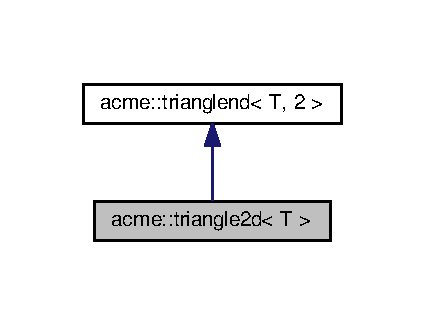
\includegraphics[width=204pt]{d8/dce/classacme_1_1triangle2d__inherit__graph}
\end{center}
\end{figure}


Collaboration diagram for acme\+:\+:triangle2d$<$ T $>$\+:
\nopagebreak
\begin{figure}[H]
\begin{center}
\leavevmode
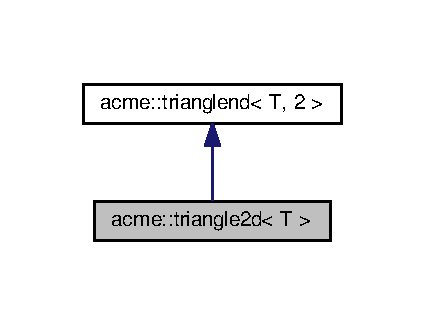
\includegraphics[width=204pt]{df/dcb/classacme_1_1triangle2d__coll__graph}
\end{center}
\end{figure}


The documentation for this class was generated from the following file\+:\begin{DoxyCompactItemize}
\item 
src/acme\+\_\+triangle.\+hh\end{DoxyCompactItemize}

\hypertarget{classacme_1_1triangle3d}{}\section{acme\+:\+:triangle3d$<$ T $>$ Class Template Reference}
\label{classacme_1_1triangle3d}\index{acme\+::triangle3d$<$ T $>$@{acme\+::triangle3d$<$ T $>$}}


Inheritance diagram for acme\+:\+:triangle3d$<$ T $>$\+:
\nopagebreak
\begin{figure}[H]
\begin{center}
\leavevmode
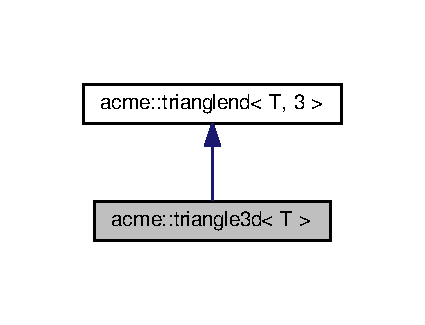
\includegraphics[width=204pt]{da/dec/classacme_1_1triangle3d__inherit__graph}
\end{center}
\end{figure}


Collaboration diagram for acme\+:\+:triangle3d$<$ T $>$\+:
\nopagebreak
\begin{figure}[H]
\begin{center}
\leavevmode
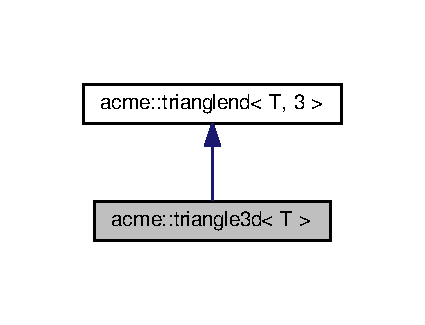
\includegraphics[width=204pt]{d7/dab/classacme_1_1triangle3d__coll__graph}
\end{center}
\end{figure}


The documentation for this class was generated from the following file\+:\begin{DoxyCompactItemize}
\item 
src/acme\+\_\+triangle.\+hh\end{DoxyCompactItemize}

\hypertarget{classacme_1_1trianglend}{}\section{acme\+:\+:trianglend$<$ T, D $>$ Class Template Reference}
\label{classacme_1_1trianglend}\index{acme\+::trianglend$<$ T, D $>$@{acme\+::trianglend$<$ T, D $>$}}


The documentation for this class was generated from the following file\+:\begin{DoxyCompactItemize}
\item 
src/acme\+\_\+triangle.\+hh\end{DoxyCompactItemize}

\hypertarget{classacme_1_1vector2d}{}\section{acme\+:\+:vector2d$<$ T $>$ Class Template Reference}
\label{classacme_1_1vector2d}\index{acme\+::vector2d$<$ T $>$@{acme\+::vector2d$<$ T $>$}}


Inheritance diagram for acme\+:\+:vector2d$<$ T $>$\+:
\nopagebreak
\begin{figure}[H]
\begin{center}
\leavevmode
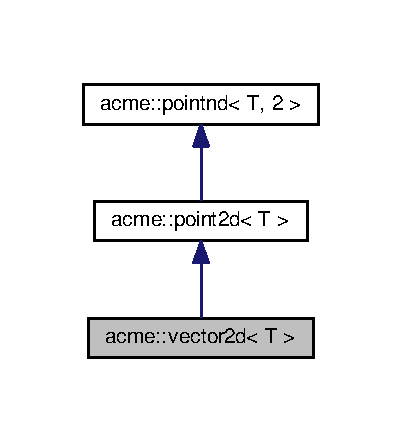
\includegraphics[width=193pt]{d1/d4a/classacme_1_1vector2d__inherit__graph}
\end{center}
\end{figure}


Collaboration diagram for acme\+:\+:vector2d$<$ T $>$\+:
\nopagebreak
\begin{figure}[H]
\begin{center}
\leavevmode
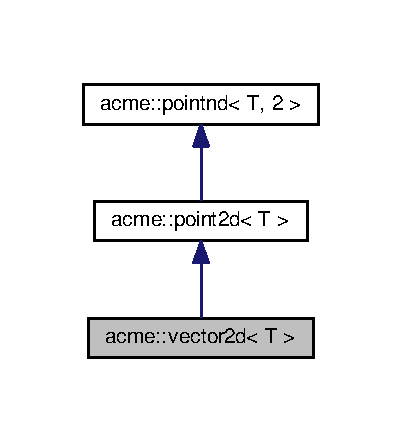
\includegraphics[width=193pt]{dd/daa/classacme_1_1vector2d__coll__graph}
\end{center}
\end{figure}
\subsection*{Public Member Functions}
\begin{DoxyCompactItemize}
\item 
\mbox{\Hypertarget{classacme_1_1vector2d_a830f86da17bb90b237e007f3ea6abb55}\label{classacme_1_1vector2d_a830f86da17bb90b237e007f3ea6abb55}} 
{\bfseries vector2d} (const T \&value0=T(0.\+0), const T \&value1=T(0.\+0))
\item 
\mbox{\Hypertarget{classacme_1_1vector2d_a316b2f73402d2cc96e3d676dab097add}\label{classacme_1_1vector2d_a316b2f73402d2cc96e3d676dab097add}} 
\hyperlink{classacme_1_1vector2d}{vector2d}$<$ T $>$ \& {\bfseries operator=} (const \hyperlink{classacme_1_1vectornd}{vectornd}$<$ T, 2 $>$ \&vector)
\item 
\mbox{\Hypertarget{classacme_1_1point2d_aa62c36149dc319bcd38b351be5230f04}\label{classacme_1_1point2d_aa62c36149dc319bcd38b351be5230f04}} 
const T \& \hyperlink{classacme_1_1point2d_aa62c36149dc319bcd38b351be5230f04}{x} () const
\begin{DoxyCompactList}\small\item\em Getter for point x value. \end{DoxyCompactList}\item 
void \hyperlink{classacme_1_1point2d_a158797a6603451c35bd0e2be3be3b2c8}{x} (const T \&x)
\begin{DoxyCompactList}\small\item\em Setter for point x value. \end{DoxyCompactList}\item 
\mbox{\Hypertarget{classacme_1_1point2d_adf79b9f2fbcac2c5f1bea2bece0e9b27}\label{classacme_1_1point2d_adf79b9f2fbcac2c5f1bea2bece0e9b27}} 
const T \& \hyperlink{classacme_1_1point2d_adf79b9f2fbcac2c5f1bea2bece0e9b27}{y} () const
\begin{DoxyCompactList}\small\item\em Getter for point y value. \end{DoxyCompactList}\item 
void \hyperlink{classacme_1_1point2d_ab1baab0e82e178f1e828a25fa8dbb1c8}{y} (const T \&y)
\begin{DoxyCompactList}\small\item\em Setter for point y value. \end{DoxyCompactList}\item 
\hyperlink{classacme_1_1point2d}{point2d}$<$ T $>$ \& \hyperlink{classacme_1_1point2d_a23948fcd0635557e8eeb0c298bb96f68}{make3dX} (const T \&\hyperlink{classacme_1_1point2d_aa62c36149dc319bcd38b351be5230f04}{x})
\begin{DoxyCompactList}\small\item\em Create a 3-\/dimensional point by addind x value. \end{DoxyCompactList}\item 
\hyperlink{classacme_1_1point2d}{point2d}$<$ T $>$ \& \hyperlink{classacme_1_1point2d_ac6bdbcec56da64ea0265691f3e734625}{make3dY} (const T \&\hyperlink{classacme_1_1point2d_adf79b9f2fbcac2c5f1bea2bece0e9b27}{y})
\begin{DoxyCompactList}\small\item\em Create a 3-\/dimensional point by addind y value. \end{DoxyCompactList}\item 
\hyperlink{classacme_1_1point2d}{point2d}$<$ T $>$ \& \hyperlink{classacme_1_1point2d_a605f4d335747c08026316ec4982b7eb5}{make3dZ} (const T \&z)
\begin{DoxyCompactList}\small\item\em Create a 3-\/dimensional point by addind z value. \end{DoxyCompactList}\item 
\mbox{\Hypertarget{classacme_1_1pointnd_a2d0b84e609dc1ad5cbbe631c5bb5791f}\label{classacme_1_1pointnd_a2d0b84e609dc1ad5cbbe631c5bb5791f}} 
void \hyperlink{classacme_1_1pointnd_a2d0b84e609dc1ad5cbbe631c5bb5791f}{clear} ()
\begin{DoxyCompactList}\small\item\em Clear vector data. \end{DoxyCompactList}\item 
T \& \hyperlink{classacme_1_1pointnd_a35b0691673728d98d455c007612d6b91}{operator\mbox{[}$\,$\mbox{]}} (const std\+::size\+\_\+t \&index)
\begin{DoxyCompactList}\small\item\em Indexing operator. \end{DoxyCompactList}\item 
const T \& \hyperlink{classacme_1_1pointnd_a565e9ed195c8f8dadc570a029a3deb94}{operator\mbox{[}$\,$\mbox{]}} (const std\+::size\+\_\+t \&index) const
\begin{DoxyCompactList}\small\item\em Indexing operator. \end{DoxyCompactList}\end{DoxyCompactItemize}
\subsection*{Protected Attributes}
\begin{DoxyCompactItemize}
\item 
\mbox{\Hypertarget{classacme_1_1pointnd_a13b19080ed617e2a9c5d6058f07d4f4b}\label{classacme_1_1pointnd_a13b19080ed617e2a9c5d6058f07d4f4b}} 
Eigen\+::\+Matrix$<$ T, D, 1 $>$ {\bfseries data}
\end{DoxyCompactItemize}


\subsection{Member Function Documentation}
\mbox{\Hypertarget{classacme_1_1point2d_a23948fcd0635557e8eeb0c298bb96f68}\label{classacme_1_1point2d_a23948fcd0635557e8eeb0c298bb96f68}} 
\index{acme\+::vector2d@{acme\+::vector2d}!make3dX@{make3dX}}
\index{make3dX@{make3dX}!acme\+::vector2d@{acme\+::vector2d}}
\subsubsection{\texorpdfstring{make3d\+X()}{make3dX()}}
{\footnotesize\ttfamily template$<$typename T = Float$>$ \\
\hyperlink{classacme_1_1point2d}{point2d}$<$T$>$\& \hyperlink{classacme_1_1point2d}{acme\+::point2d}$<$ T $>$\+::make3dX (\begin{DoxyParamCaption}\item[{const T \&}]{x }\end{DoxyParamCaption})\hspace{0.3cm}{\ttfamily [inline]}, {\ttfamily [inherited]}}



Create a 3-\/dimensional point by addind x value. 


\begin{DoxyParams}{Parameters}
{\em x} & Input x value \\
\hline
\end{DoxyParams}
\mbox{\Hypertarget{classacme_1_1point2d_ac6bdbcec56da64ea0265691f3e734625}\label{classacme_1_1point2d_ac6bdbcec56da64ea0265691f3e734625}} 
\index{acme\+::vector2d@{acme\+::vector2d}!make3dY@{make3dY}}
\index{make3dY@{make3dY}!acme\+::vector2d@{acme\+::vector2d}}
\subsubsection{\texorpdfstring{make3d\+Y()}{make3dY()}}
{\footnotesize\ttfamily template$<$typename T = Float$>$ \\
\hyperlink{classacme_1_1point2d}{point2d}$<$T$>$\& \hyperlink{classacme_1_1point2d}{acme\+::point2d}$<$ T $>$\+::make3dY (\begin{DoxyParamCaption}\item[{const T \&}]{y }\end{DoxyParamCaption})\hspace{0.3cm}{\ttfamily [inline]}, {\ttfamily [inherited]}}



Create a 3-\/dimensional point by addind y value. 


\begin{DoxyParams}{Parameters}
{\em y} & Input y value \\
\hline
\end{DoxyParams}
\mbox{\Hypertarget{classacme_1_1point2d_a605f4d335747c08026316ec4982b7eb5}\label{classacme_1_1point2d_a605f4d335747c08026316ec4982b7eb5}} 
\index{acme\+::vector2d@{acme\+::vector2d}!make3dZ@{make3dZ}}
\index{make3dZ@{make3dZ}!acme\+::vector2d@{acme\+::vector2d}}
\subsubsection{\texorpdfstring{make3d\+Z()}{make3dZ()}}
{\footnotesize\ttfamily template$<$typename T = Float$>$ \\
\hyperlink{classacme_1_1point2d}{point2d}$<$T$>$\& \hyperlink{classacme_1_1point2d}{acme\+::point2d}$<$ T $>$\+::make3dZ (\begin{DoxyParamCaption}\item[{const T \&}]{z }\end{DoxyParamCaption})\hspace{0.3cm}{\ttfamily [inline]}, {\ttfamily [inherited]}}



Create a 3-\/dimensional point by addind z value. 


\begin{DoxyParams}{Parameters}
{\em z} & Input z value \\
\hline
\end{DoxyParams}
\mbox{\Hypertarget{classacme_1_1pointnd_a35b0691673728d98d455c007612d6b91}\label{classacme_1_1pointnd_a35b0691673728d98d455c007612d6b91}} 
\index{acme\+::vector2d@{acme\+::vector2d}!operator\mbox{[}\mbox{]}@{operator[]}}
\index{operator\mbox{[}\mbox{]}@{operator[]}!acme\+::vector2d@{acme\+::vector2d}}
\subsubsection{\texorpdfstring{operator[]()}{operator[]()}\hspace{0.1cm}{\footnotesize\ttfamily [1/2]}}
{\footnotesize\ttfamily T\& \hyperlink{classacme_1_1pointnd}{acme\+::pointnd}$<$ T, D $>$\+::operator\mbox{[}$\,$\mbox{]} (\begin{DoxyParamCaption}\item[{const std\+::size\+\_\+t \&}]{index }\end{DoxyParamCaption})\hspace{0.3cm}{\ttfamily [inline]}, {\ttfamily [inherited]}}



Indexing operator. 


\begin{DoxyParams}{Parameters}
{\em index} & Input index \\
\hline
\end{DoxyParams}
\mbox{\Hypertarget{classacme_1_1pointnd_a565e9ed195c8f8dadc570a029a3deb94}\label{classacme_1_1pointnd_a565e9ed195c8f8dadc570a029a3deb94}} 
\index{acme\+::vector2d@{acme\+::vector2d}!operator\mbox{[}\mbox{]}@{operator[]}}
\index{operator\mbox{[}\mbox{]}@{operator[]}!acme\+::vector2d@{acme\+::vector2d}}
\subsubsection{\texorpdfstring{operator[]()}{operator[]()}\hspace{0.1cm}{\footnotesize\ttfamily [2/2]}}
{\footnotesize\ttfamily const T\& \hyperlink{classacme_1_1pointnd}{acme\+::pointnd}$<$ T, D $>$\+::operator\mbox{[}$\,$\mbox{]} (\begin{DoxyParamCaption}\item[{const std\+::size\+\_\+t \&}]{index }\end{DoxyParamCaption}) const\hspace{0.3cm}{\ttfamily [inline]}, {\ttfamily [inherited]}}



Indexing operator. 


\begin{DoxyParams}{Parameters}
{\em index} & Input index \\
\hline
\end{DoxyParams}
\mbox{\Hypertarget{classacme_1_1point2d_a158797a6603451c35bd0e2be3be3b2c8}\label{classacme_1_1point2d_a158797a6603451c35bd0e2be3be3b2c8}} 
\index{acme\+::vector2d@{acme\+::vector2d}!x@{x}}
\index{x@{x}!acme\+::vector2d@{acme\+::vector2d}}
\subsubsection{\texorpdfstring{x()}{x()}}
{\footnotesize\ttfamily template$<$typename T = Float$>$ \\
void \hyperlink{classacme_1_1point2d}{acme\+::point2d}$<$ T $>$\+::x (\begin{DoxyParamCaption}\item[{const T \&}]{x }\end{DoxyParamCaption})\hspace{0.3cm}{\ttfamily [inline]}, {\ttfamily [inherited]}}



Setter for point x value. 


\begin{DoxyParams}{Parameters}
{\em x} & Input x value \\
\hline
\end{DoxyParams}
\mbox{\Hypertarget{classacme_1_1point2d_ab1baab0e82e178f1e828a25fa8dbb1c8}\label{classacme_1_1point2d_ab1baab0e82e178f1e828a25fa8dbb1c8}} 
\index{acme\+::vector2d@{acme\+::vector2d}!y@{y}}
\index{y@{y}!acme\+::vector2d@{acme\+::vector2d}}
\subsubsection{\texorpdfstring{y()}{y()}}
{\footnotesize\ttfamily template$<$typename T = Float$>$ \\
void \hyperlink{classacme_1_1point2d}{acme\+::point2d}$<$ T $>$\+::y (\begin{DoxyParamCaption}\item[{const T \&}]{y }\end{DoxyParamCaption})\hspace{0.3cm}{\ttfamily [inline]}, {\ttfamily [inherited]}}



Setter for point y value. 


\begin{DoxyParams}{Parameters}
{\em y} & Input y value \\
\hline
\end{DoxyParams}


The documentation for this class was generated from the following file\+:\begin{DoxyCompactItemize}
\item 
src/acme\+\_\+vector.\+hh\end{DoxyCompactItemize}

\hypertarget{classacme_1_1vector3d}{}\section{acme\+:\+:vector3d$<$ T $>$ Class Template Reference}
\label{classacme_1_1vector3d}\index{acme\+::vector3d$<$ T $>$@{acme\+::vector3d$<$ T $>$}}


Inheritance diagram for acme\+:\+:vector3d$<$ T $>$\+:
\nopagebreak
\begin{figure}[H]
\begin{center}
\leavevmode
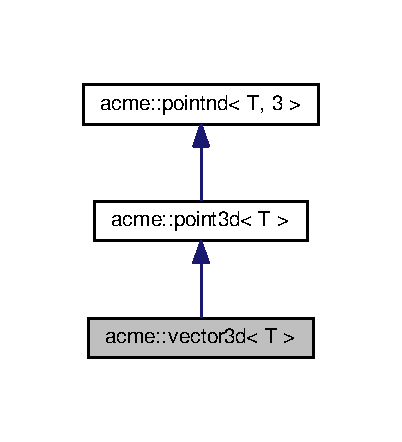
\includegraphics[width=193pt]{d1/d53/classacme_1_1vector3d__inherit__graph}
\end{center}
\end{figure}


Collaboration diagram for acme\+:\+:vector3d$<$ T $>$\+:
\nopagebreak
\begin{figure}[H]
\begin{center}
\leavevmode
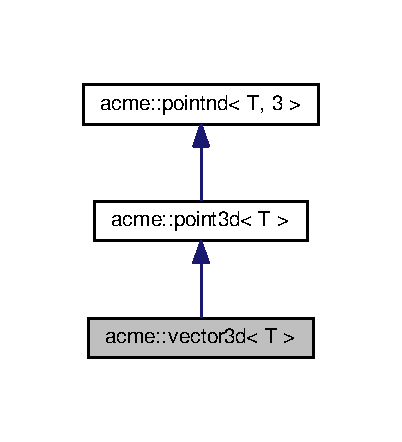
\includegraphics[width=193pt]{d0/d2c/classacme_1_1vector3d__coll__graph}
\end{center}
\end{figure}
\subsection*{Public Member Functions}
\begin{DoxyCompactItemize}
\item 
\mbox{\Hypertarget{classacme_1_1vector3d_a93f7fa7c6419cccf56333d909cc1d51e}\label{classacme_1_1vector3d_a93f7fa7c6419cccf56333d909cc1d51e}} 
{\bfseries vector3d} (const T \&value0=T(0.\+0), const T \&value1=T(0.\+0), const T \&value2=T(0.\+0))
\item 
\mbox{\Hypertarget{classacme_1_1vector3d_a2668398e02c44822585f3bef70ab3645}\label{classacme_1_1vector3d_a2668398e02c44822585f3bef70ab3645}} 
\hyperlink{classacme_1_1vector3d}{vector3d}$<$ T $>$ \& {\bfseries operator=} (const \hyperlink{classacme_1_1vectornd}{vectornd}$<$ T, 3 $>$ \&vector)
\item 
\mbox{\Hypertarget{classacme_1_1point3d_a7ace84b8e85e0762e8c900ef7dfabf61}\label{classacme_1_1point3d_a7ace84b8e85e0762e8c900ef7dfabf61}} 
const T \& \hyperlink{classacme_1_1point3d_a7ace84b8e85e0762e8c900ef7dfabf61}{x} () const
\begin{DoxyCompactList}\small\item\em Getter for point x value. \end{DoxyCompactList}\item 
void \hyperlink{classacme_1_1point3d_acccc28f082747904be0f39bd5972a40e}{x} (const T \&x)
\begin{DoxyCompactList}\small\item\em Setter for point x value. \end{DoxyCompactList}\item 
\mbox{\Hypertarget{classacme_1_1point3d_a1a13aea2bb5e756c74ca6187e4b927d2}\label{classacme_1_1point3d_a1a13aea2bb5e756c74ca6187e4b927d2}} 
const T \& \hyperlink{classacme_1_1point3d_a1a13aea2bb5e756c74ca6187e4b927d2}{y} () const
\begin{DoxyCompactList}\small\item\em Getter for point y value. \end{DoxyCompactList}\item 
void \hyperlink{classacme_1_1point3d_ad9b058b4ba5ca4172a8c4ded27c89825}{y} (const T \&y)
\begin{DoxyCompactList}\small\item\em Setter for point y value. \end{DoxyCompactList}\item 
\mbox{\Hypertarget{classacme_1_1point3d_acbea0b411604f8da4f690e09e2401743}\label{classacme_1_1point3d_acbea0b411604f8da4f690e09e2401743}} 
const T \& \hyperlink{classacme_1_1point3d_acbea0b411604f8da4f690e09e2401743}{z} () const
\begin{DoxyCompactList}\small\item\em Getter for point z value. \end{DoxyCompactList}\item 
void \hyperlink{classacme_1_1point3d_aad69f4d32ffafffd008214c361fa843f}{z} (const T \&z)
\begin{DoxyCompactList}\small\item\em Setter for point z value. \end{DoxyCompactList}\item 
\hyperlink{classacme_1_1point2d}{point2d}$<$ T $>$ \& \hyperlink{classacme_1_1point3d_a724a96c6ad4aa84b0236a8113d99d4a4}{make2d} (const std\+::size\+\_\+t \&index1, const std\+::size\+\_\+t \&index2)
\begin{DoxyCompactList}\small\item\em Create a 3-\/dimensional point by addind value on selected index value. \end{DoxyCompactList}\item 
\mbox{\Hypertarget{classacme_1_1pointnd_a2d0b84e609dc1ad5cbbe631c5bb5791f}\label{classacme_1_1pointnd_a2d0b84e609dc1ad5cbbe631c5bb5791f}} 
void \hyperlink{classacme_1_1pointnd_a2d0b84e609dc1ad5cbbe631c5bb5791f}{clear} ()
\begin{DoxyCompactList}\small\item\em Clear vector data. \end{DoxyCompactList}\item 
T \& \hyperlink{classacme_1_1pointnd_a35b0691673728d98d455c007612d6b91}{operator\mbox{[}$\,$\mbox{]}} (const std\+::size\+\_\+t \&index)
\begin{DoxyCompactList}\small\item\em Indexing operator. \end{DoxyCompactList}\item 
const T \& \hyperlink{classacme_1_1pointnd_a565e9ed195c8f8dadc570a029a3deb94}{operator\mbox{[}$\,$\mbox{]}} (const std\+::size\+\_\+t \&index) const
\begin{DoxyCompactList}\small\item\em Indexing operator. \end{DoxyCompactList}\end{DoxyCompactItemize}
\subsection*{Protected Attributes}
\begin{DoxyCompactItemize}
\item 
\mbox{\Hypertarget{classacme_1_1pointnd_a13b19080ed617e2a9c5d6058f07d4f4b}\label{classacme_1_1pointnd_a13b19080ed617e2a9c5d6058f07d4f4b}} 
Eigen\+::\+Matrix$<$ T, D, 1 $>$ {\bfseries data}
\end{DoxyCompactItemize}


\subsection{Member Function Documentation}
\mbox{\Hypertarget{classacme_1_1point3d_a724a96c6ad4aa84b0236a8113d99d4a4}\label{classacme_1_1point3d_a724a96c6ad4aa84b0236a8113d99d4a4}} 
\index{acme\+::vector3d@{acme\+::vector3d}!make2d@{make2d}}
\index{make2d@{make2d}!acme\+::vector3d@{acme\+::vector3d}}
\subsubsection{\texorpdfstring{make2d()}{make2d()}}
{\footnotesize\ttfamily template$<$typename T = Float$>$ \\
\hyperlink{classacme_1_1point2d}{point2d}$<$T$>$\& \hyperlink{classacme_1_1point3d}{acme\+::point3d}$<$ T $>$\+::make2d (\begin{DoxyParamCaption}\item[{const std\+::size\+\_\+t \&}]{index1,  }\item[{const std\+::size\+\_\+t \&}]{index2 }\end{DoxyParamCaption})\hspace{0.3cm}{\ttfamily [inline]}, {\ttfamily [inherited]}}



Create a 3-\/dimensional point by addind value on selected index value. 


\begin{DoxyParams}{Parameters}
{\em index1} & Inuput index 1 \\
\hline
{\em index2} & Inuput index 2 \\
\hline
\end{DoxyParams}
\mbox{\Hypertarget{classacme_1_1pointnd_a35b0691673728d98d455c007612d6b91}\label{classacme_1_1pointnd_a35b0691673728d98d455c007612d6b91}} 
\index{acme\+::vector3d@{acme\+::vector3d}!operator\mbox{[}\mbox{]}@{operator[]}}
\index{operator\mbox{[}\mbox{]}@{operator[]}!acme\+::vector3d@{acme\+::vector3d}}
\subsubsection{\texorpdfstring{operator[]()}{operator[]()}\hspace{0.1cm}{\footnotesize\ttfamily [1/2]}}
{\footnotesize\ttfamily T\& \hyperlink{classacme_1_1pointnd}{acme\+::pointnd}$<$ T, D $>$\+::operator\mbox{[}$\,$\mbox{]} (\begin{DoxyParamCaption}\item[{const std\+::size\+\_\+t \&}]{index }\end{DoxyParamCaption})\hspace{0.3cm}{\ttfamily [inline]}, {\ttfamily [inherited]}}



Indexing operator. 


\begin{DoxyParams}{Parameters}
{\em index} & Input index \\
\hline
\end{DoxyParams}
\mbox{\Hypertarget{classacme_1_1pointnd_a565e9ed195c8f8dadc570a029a3deb94}\label{classacme_1_1pointnd_a565e9ed195c8f8dadc570a029a3deb94}} 
\index{acme\+::vector3d@{acme\+::vector3d}!operator\mbox{[}\mbox{]}@{operator[]}}
\index{operator\mbox{[}\mbox{]}@{operator[]}!acme\+::vector3d@{acme\+::vector3d}}
\subsubsection{\texorpdfstring{operator[]()}{operator[]()}\hspace{0.1cm}{\footnotesize\ttfamily [2/2]}}
{\footnotesize\ttfamily const T\& \hyperlink{classacme_1_1pointnd}{acme\+::pointnd}$<$ T, D $>$\+::operator\mbox{[}$\,$\mbox{]} (\begin{DoxyParamCaption}\item[{const std\+::size\+\_\+t \&}]{index }\end{DoxyParamCaption}) const\hspace{0.3cm}{\ttfamily [inline]}, {\ttfamily [inherited]}}



Indexing operator. 


\begin{DoxyParams}{Parameters}
{\em index} & Input index \\
\hline
\end{DoxyParams}
\mbox{\Hypertarget{classacme_1_1point3d_acccc28f082747904be0f39bd5972a40e}\label{classacme_1_1point3d_acccc28f082747904be0f39bd5972a40e}} 
\index{acme\+::vector3d@{acme\+::vector3d}!x@{x}}
\index{x@{x}!acme\+::vector3d@{acme\+::vector3d}}
\subsubsection{\texorpdfstring{x()}{x()}}
{\footnotesize\ttfamily template$<$typename T = Float$>$ \\
void \hyperlink{classacme_1_1point3d}{acme\+::point3d}$<$ T $>$\+::x (\begin{DoxyParamCaption}\item[{const T \&}]{x }\end{DoxyParamCaption})\hspace{0.3cm}{\ttfamily [inline]}, {\ttfamily [inherited]}}



Setter for point x value. 


\begin{DoxyParams}{Parameters}
{\em x} & Input x value \\
\hline
\end{DoxyParams}
\mbox{\Hypertarget{classacme_1_1point3d_ad9b058b4ba5ca4172a8c4ded27c89825}\label{classacme_1_1point3d_ad9b058b4ba5ca4172a8c4ded27c89825}} 
\index{acme\+::vector3d@{acme\+::vector3d}!y@{y}}
\index{y@{y}!acme\+::vector3d@{acme\+::vector3d}}
\subsubsection{\texorpdfstring{y()}{y()}}
{\footnotesize\ttfamily template$<$typename T = Float$>$ \\
void \hyperlink{classacme_1_1point3d}{acme\+::point3d}$<$ T $>$\+::y (\begin{DoxyParamCaption}\item[{const T \&}]{y }\end{DoxyParamCaption})\hspace{0.3cm}{\ttfamily [inline]}, {\ttfamily [inherited]}}



Setter for point y value. 


\begin{DoxyParams}{Parameters}
{\em y} & Input y value \\
\hline
\end{DoxyParams}
\mbox{\Hypertarget{classacme_1_1point3d_aad69f4d32ffafffd008214c361fa843f}\label{classacme_1_1point3d_aad69f4d32ffafffd008214c361fa843f}} 
\index{acme\+::vector3d@{acme\+::vector3d}!z@{z}}
\index{z@{z}!acme\+::vector3d@{acme\+::vector3d}}
\subsubsection{\texorpdfstring{z()}{z()}}
{\footnotesize\ttfamily template$<$typename T = Float$>$ \\
void \hyperlink{classacme_1_1point3d}{acme\+::point3d}$<$ T $>$\+::z (\begin{DoxyParamCaption}\item[{const T \&}]{z }\end{DoxyParamCaption})\hspace{0.3cm}{\ttfamily [inline]}, {\ttfamily [inherited]}}



Setter for point z value. 


\begin{DoxyParams}{Parameters}
{\em z} & Input z value \\
\hline
\end{DoxyParams}


The documentation for this class was generated from the following file\+:\begin{DoxyCompactItemize}
\item 
src/acme\+\_\+vector.\+hh\end{DoxyCompactItemize}

\hypertarget{classacme_1_1vectornd}{}\section{acme\+:\+:vectornd$<$ T, D $>$ Class Template Reference}
\label{classacme_1_1vectornd}\index{acme\+::vectornd$<$ T, D $>$@{acme\+::vectornd$<$ T, D $>$}}


Inheritance diagram for acme\+:\+:vectornd$<$ T, D $>$\+:
\nopagebreak
\begin{figure}[H]
\begin{center}
\leavevmode
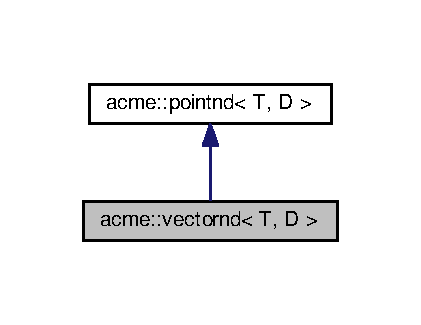
\includegraphics[width=202pt]{dc/df5/classacme_1_1vectornd__inherit__graph}
\end{center}
\end{figure}


Collaboration diagram for acme\+:\+:vectornd$<$ T, D $>$\+:
\nopagebreak
\begin{figure}[H]
\begin{center}
\leavevmode
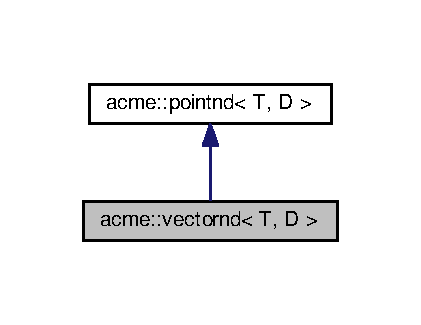
\includegraphics[width=202pt]{d8/d02/classacme_1_1vectornd__coll__graph}
\end{center}
\end{figure}
\subsection*{Public Member Functions}
\begin{DoxyCompactItemize}
\item 
\mbox{\Hypertarget{classacme_1_1vectornd_ab5dc63b6b6930829fd1be72fbbb3e2cb}\label{classacme_1_1vectornd_ab5dc63b6b6930829fd1be72fbbb3e2cb}} 
{\bfseries vectornd} (const T \&v0)
\item 
\mbox{\Hypertarget{classacme_1_1vectornd_ad5b21158841bed8eef52d240ba6c892d}\label{classacme_1_1vectornd_ad5b21158841bed8eef52d240ba6c892d}} 
{\bfseries vectornd} (const T \&v0, const T \&v1)
\item 
\mbox{\Hypertarget{classacme_1_1vectornd_a5e1fc35ace1eb455ea043272bc7fcd39}\label{classacme_1_1vectornd_a5e1fc35ace1eb455ea043272bc7fcd39}} 
{\bfseries vectornd} (const T \&v0, const T \&v1, const T \&v2)
\item 
\mbox{\Hypertarget{classacme_1_1vectornd_a71cffdc32a6e041af16fa0db477d8ec7}\label{classacme_1_1vectornd_a71cffdc32a6e041af16fa0db477d8ec7}} 
{\bfseries vectornd} (const T \&v0, const T \&v1, const T \&v2, const T \&v3)
\item 
\mbox{\Hypertarget{classacme_1_1vectornd_a990e311e894b7a8ac9954597844c2991}\label{classacme_1_1vectornd_a990e311e894b7a8ac9954597844c2991}} 
{\bfseries vectornd} (const \hyperlink{classacme_1_1vectornd}{vectornd}$<$ T, D $>$ \&vector)
\item 
\mbox{\Hypertarget{classacme_1_1pointnd_a2d0b84e609dc1ad5cbbe631c5bb5791f}\label{classacme_1_1pointnd_a2d0b84e609dc1ad5cbbe631c5bb5791f}} 
void \hyperlink{classacme_1_1pointnd_a2d0b84e609dc1ad5cbbe631c5bb5791f}{clear} ()
\begin{DoxyCompactList}\small\item\em Clear vector data. \end{DoxyCompactList}\item 
T \& \hyperlink{classacme_1_1pointnd_a35b0691673728d98d455c007612d6b91}{operator\mbox{[}$\,$\mbox{]}} (const std\+::size\+\_\+t \&index)
\begin{DoxyCompactList}\small\item\em Indexing operator. \end{DoxyCompactList}\item 
const T \& \hyperlink{classacme_1_1pointnd_a565e9ed195c8f8dadc570a029a3deb94}{operator\mbox{[}$\,$\mbox{]}} (const std\+::size\+\_\+t \&index) const
\begin{DoxyCompactList}\small\item\em Indexing operator. \end{DoxyCompactList}\end{DoxyCompactItemize}
\subsection*{Protected Attributes}
\begin{DoxyCompactItemize}
\item 
\mbox{\Hypertarget{classacme_1_1pointnd_a13b19080ed617e2a9c5d6058f07d4f4b}\label{classacme_1_1pointnd_a13b19080ed617e2a9c5d6058f07d4f4b}} 
Eigen\+::\+Matrix$<$ T, D, 1 $>$ {\bfseries data}
\end{DoxyCompactItemize}


\subsection{Member Function Documentation}
\mbox{\Hypertarget{classacme_1_1pointnd_a35b0691673728d98d455c007612d6b91}\label{classacme_1_1pointnd_a35b0691673728d98d455c007612d6b91}} 
\index{acme\+::vectornd@{acme\+::vectornd}!operator\mbox{[}\mbox{]}@{operator[]}}
\index{operator\mbox{[}\mbox{]}@{operator[]}!acme\+::vectornd@{acme\+::vectornd}}
\subsubsection{\texorpdfstring{operator[]()}{operator[]()}\hspace{0.1cm}{\footnotesize\ttfamily [1/2]}}
{\footnotesize\ttfamily template$<$typename T, std\+::size\+\_\+t D$>$ \\
T\& \hyperlink{classacme_1_1pointnd}{acme\+::pointnd}$<$ T, D $>$\+::operator\mbox{[}$\,$\mbox{]} (\begin{DoxyParamCaption}\item[{const std\+::size\+\_\+t \&}]{index }\end{DoxyParamCaption})\hspace{0.3cm}{\ttfamily [inline]}, {\ttfamily [inherited]}}



Indexing operator. 


\begin{DoxyParams}{Parameters}
{\em index} & Input index \\
\hline
\end{DoxyParams}
\mbox{\Hypertarget{classacme_1_1pointnd_a565e9ed195c8f8dadc570a029a3deb94}\label{classacme_1_1pointnd_a565e9ed195c8f8dadc570a029a3deb94}} 
\index{acme\+::vectornd@{acme\+::vectornd}!operator\mbox{[}\mbox{]}@{operator[]}}
\index{operator\mbox{[}\mbox{]}@{operator[]}!acme\+::vectornd@{acme\+::vectornd}}
\subsubsection{\texorpdfstring{operator[]()}{operator[]()}\hspace{0.1cm}{\footnotesize\ttfamily [2/2]}}
{\footnotesize\ttfamily template$<$typename T, std\+::size\+\_\+t D$>$ \\
const T\& \hyperlink{classacme_1_1pointnd}{acme\+::pointnd}$<$ T, D $>$\+::operator\mbox{[}$\,$\mbox{]} (\begin{DoxyParamCaption}\item[{const std\+::size\+\_\+t \&}]{index }\end{DoxyParamCaption}) const\hspace{0.3cm}{\ttfamily [inline]}, {\ttfamily [inherited]}}



Indexing operator. 


\begin{DoxyParams}{Parameters}
{\em index} & Input index \\
\hline
\end{DoxyParams}


The documentation for this class was generated from the following file\+:\begin{DoxyCompactItemize}
\item 
src/acme\+\_\+vector.\+hh\end{DoxyCompactItemize}

%--- End generated contents ---

% Index
\backmatter
\newpage
\phantomsection
\clearemptydoublepage
\addcontentsline{toc}{chapter}{Index}
\printindex

\end{document}
